\documentclass[12pt]{article}

% Packages
\usepackage{amsmath, amssymb, amsfonts}
\usepackage{fullpage}
\usepackage{hyperref}
\usepackage{cite}
\usepackage{graphicx}
\usepackage{booktabs}
\usepackage{float}
\usepackage{enumitem}
\usepackage{etoolbox}
\usepackage[justification=justified,singlelinecheck=false]{caption}
\setlength{\parindent}{0pt}
\setlist[itemize]{leftmargin=0pt,itemindent=0pt,listparindent=0pt}
\captionsetup{margin=0pt,indention=0pt}
% Keep prose flush with the text margin, including special environments.
\patchcmd{\abstract}{\quotation}{}{}
  {\PackageError{survey}{Abstract alignment patch failed}{}}
\patchcmd{\endabstract}{\endquotation}{}{}
  {\PackageError{survey}{Abstract alignment patch failed}{}}
\patchcmd{\thebibliography}{\leftmargin\labelwidth}
  {\leftmargin0pt\labelwidth0pt\itemindent\labelsep
   \let\makelabel\textnormal}{}
  {\PackageError{survey}{Bibliography alignment patch failed}{}}
\patchcmd{\thebibliography}{\advance\leftmargin\labelsep}
  {}{}
  {\PackageError{survey}{Bibliography alignment patch failed}{}}
\hypersetup{hypertexnames=false}

% This block creates the .bib file automatically with the references
\begin{filecontents}{references.bib}
@article{BDL,
  title={From sparse solutions of systems of equations to sparse modeling of signals and images},
  author={Bruckstein, Alfred M and Donoho, David L and Elad, Michael},
  journal={SIAM Review},
  volume={51},
  number={1},
  pages={34--81},
  year={2009},
  publisher={SIAM}
}

@article{Baraniuk,
  title={Model-based compressive sensing},
  author={Baraniuk, Richard G and Cevher, Volkan and Duarte, Marco F and Hegde, Chinmay},
  journal={IEEE Transactions on Information Theory},
  volume={56},
  number={4},
  pages={1982--2001},
  year={2010},
  publisher={IEEE}
}

@article{Ozay,
  title={Sparse malicious false data injection attacks and defense mechanisms in smart grids},
  author={Ozay, Mete and Esnaola, Inaki and Vural, Fatos T Yarman and Kulkarni, Sanjeev R and Poor, H Vincent},
  journal={IEEE Transactions on Smart Grid},
  volume={7},
  number={6},
  pages={2744--2755},
  year={2016},
  publisher={IEEE}
}

@article{XuLGSR,
  title={Approximately locality-constrained group sparse representation for robust face recognition},
  author={Xu, Yong and Zhang, Zhong and Lu, Guangming and Yang, Jian},
  journal={Pattern Recognition},
  volume={47},
  number={8},
  pages={2746--2754},
  year={2014},
  publisher={Elsevier}
}

@article{GLHAD,
  title={GLHAD: Group-Lasso Hybrid Attack Detector for Multistage Manufacturing Systems},
  author={Kokhahi, F and Li, Z},
  journal={ASME Journal of Computing and Information Science in Engineering},
  volume={24},
  number={3},
  year={2024},
  publisher={American Society of Mechanical Engineers}
}

@article{Mardani,
  title={Dynamic anomalography: Tracking network anomalies via sparsity and low rank},
  author={Mardani, Morteza and Mateos, Gonzalo and Giannakis, Georgios B},
  journal={IEEE Journal of Selected Topics in Signal Processing},
  volume={7},
  number={1},
  pages={50--66},
  year={2013},
  publisher={IEEE}
}

@inproceedings{ChaoLGSR,
  title={Locality-constrained group sparse representation for robust face recognition},
  author={Chao, Yin-Wen and Yeh, Yi-Ren and Chen, Yu-Wen and Lee, Yuh-Jye and Wang, Yu-Chiang Frank},
  booktitle={2011 18th IEEE International Conference on Image Processing},
  pages={761--764},
  year={2011},
  organization={IEEE}
}

@techreport{Yadav2010,
  title={Detecting algorithmically generated malicious domain names},
  author={Yadav, Sandeep and Reddy, Ashwath KK and Reddy, AL Narasimha and Ranjan, Supranamaya},
  year={2010},
  institution={Texas A\&M University},
  note={Technical Report}
}
@article{Tseng2001,
  author={Tseng, Paul},
  title={Convergence of a Block Coordinate Descent Method for Nondifferentiable Minimization},
  journal={Journal of Optimization Theory and Applications},
  volume={109},
  number={3},
  pages={475--494},
  year={2001},
  doi={10.1023/A:1017501703105}
}
@article{YuanLin2006,
  author={Yuan, Ming and Lin, Yi},
  title={Model selection and estimation in regression with grouped variables},
  journal={Journal of the Royal Statistical Society: Series B},
  volume={68},
  number={1},
  pages={49--67},
  year={2006},
  doi={10.1111/j.1467-9868.2005.00532.x}
}
@misc{CICIDS2017,
  author={{Canadian Institute for Cybersecurity}},
  title={Intrusion Detection Evaluation Dataset (CICIDS2017)},
  year={2017},
  howpublished={\url{https://www.unb.ca/cic/datasets/ids-2017.html}}
}
\end{filecontents}
\title{\textbf{Survey on Group Sparsity in Security Applications}}
\author{Itay Shorian \\ Advisor: Dr.\ Nadav Hallak}
\date{11 December 2025}
\begin{document}
\maketitle
\begin{abstract}
\noindent
This survey reviews the application of Group Sparsity in security-oriented systems. We classify applications into four domains: Cyber-Physical Systems, Network Traffic Analysis, Smart Grids, and Biometric Security. For each domain, we present the mathematical formulation, the optimization model, and the algorithmic solution utilized to detect and mitigate threats. Additionally, we discuss emerging applications in detecting algorithmically generated malicious domains.
\end{abstract}

\section{Introduction}

Group sparsity has become an important modeling tool in security-oriented systems such as cyber-physical infrastructures, communication networks, and power grids. These systems often exhibit anomalies or attacks that are not isolated to individual measurements but instead affect entire functional subsystems. This motivates the use of structured sparsity models that operate over predefined groups of variables. The objective of this report is to outline the concepts of sparsity and group sparsity and to examine representative uses of these models in security applications.

\section{Sparse Optimization}

Let $x \in \mathbb{R}^n$. The sparsity of $x$ is defined through the cardinality of its support,
\[
\|x\|_0 = |\{\, i : x_i \neq 0 \,\}|.
\]
Sparse optimization refers to problems that incorporate such structure, typically of the form
\[
\min_{x} \; f(x) \quad \text{subject to} \quad \|x\|_0 \le k.
\]
Problems of this type arise in high-dimensional inference, compressed sensing, anomaly detection, regression, and inverse problems, as comprehensively reviewed by Bruckstein et al.~\cite{BDL}. However, the $\ell_0$ constraint is nonconvex and generally intractable, motivating the use of surrogate formulations.

\subsection{Convex Relaxation}

A common relaxation replaces $\ell_0$ with the convex $\ell_1$ norm,
\[
\min_x \; f(x) + \lambda \|x\|_1.
\]
Under appropriate conditions on the measurement operator (such as the Restricted Isometry Property), solutions to this relaxation recover the same support as those to the original $\ell_0$ problem~\cite{BDL}. This principle forms the basis of many modern methods in sparse regression.


\subsection{Structured Sparsity}

While standard sparsity models encourage solutions with few nonzero entries, many modern applications involve variables that exhibit correlations or belong to meaningful subsets. In such settings, enforcing sparsity at the individual-coordinate level is often suboptimal, as it ignores known structure in the problem. This motivates the concept of \textit{structured sparsity}~\cite{Baraniuk}.
Formally, let the support of a vector $x \in \mathbb{R}^n$ be defined as the set of indices corresponding to nonzero entries:
\[
    \text{supp}(x) = \{ i \in \{1,\dots,n\} : x_i \neq 0 \}.
\]
In standard $k$-sparsity, the support is allowed to be any subset of cardinality $k$. In contrast, structured sparsity restricts the support to belong to a specific family of allowed patterns, denoted by $\mathbb{M}$. A vector $x$ is said to satisfy the structured sparsity model if:
\[
    \text{supp}(x) \in \mathbb{M}.
\]
This generally implies that the nonzero coefficients must appear in specific configurations, effectively constraining $x$ to lie in a union of low-dimensional subspaces defined by $\mathbb{M}$.
Let $\mathcal{G} = \{G_1, \dots, G_m\}$ be a collection of groups describing these patterns. Typical examples include:
\begin{itemize}
    \item \textbf{Group sparsity:} The allowed supports are unions of a small number of disjoint groups.
    \item \textbf{Tree-structured sparsity:} Nonzero entries must follow a rooted hierarchy (e.g., if a node is nonzero, its parent must also be nonzero).
    \item \textbf{Graph sparsity:} The support must form a connected subgraph over an underlying topology.
\end{itemize}
Structured sparsity is typically enforced by replacing the $\ell_1$ norm with structured norms (such as the $\ell_{2,1}$ norm) that penalize deviations from the allowed patterns $\mathbb{M}$.

\section{Group Sparsity}

Consider a partition of the index set $\{1,\dots,n\}$ into $m$ disjoint groups $\mathcal{G} = \{G_1, \dots, G_m\}$, where $G_i \subseteq \{1,\dots,n\}$.
A vector $x$ is said to be \textit{group-sparse} if the sub-vectors $x_{G_i}$ are identically zero for the majority of groups (i.e., $x_{G_i} = 0$ for most $i$).
To promote this structure, we utilize the mixed $\ell_{2,1}$-norm (Group-Lasso penalty), defined as the sum of the Euclidean norms of the sub-vectors:
\[
\|x\|_{2,1} = \sum_{i=1}^m \|x_{G_i}\|_2.
\]
The recovery of group-sparse signals is achieved by solving the convex optimization problem:
\[
\min_{x} \; f(x) + \lambda \sum_{i=1}^m \|x_{G_i}\|_2,
\]
where $f(x)$ represents a convex loss function (such as the squared error) measuring the data fidelity, and $\lambda$ is a regularization parameter. As discussed in model-based compressive sensing frameworks~\cite{Baraniuk}, the non-differentiability of the term $\|x_{G_i}\|_2$ at zero forces the entire block $x_{G_i}$ to zero simultaneously when its contribution is insignificant, thereby enforcing the group structure.

\section{Security Applications of Group Sparsity}

Structured sparsity plays an increasingly important role in detecting, characterizing, and mitigating security threats in large-scale engineered systems. We examine several representative applications.

\subsection{Cyber-Physical Manufacturing Systems}

In multistage manufacturing systems, identifying the source of a fault is challenging because errors propagate downstream. Malicious False Data Injection (FDI) attacks or component failures in one stage affect quality measurements in all subsequent stages. This dependency creates a \textit{grouped} structure in the error vector.
The relationship between quality measurements $y$ and the fault sources $u$ is modeled via a Stream of Variation (SoV) state-space model, often reduced to a linear form $y = \Phi u + v$. Kokhahi and Li~\cite{GLHAD} formulate the fault isolation problem as a Group Lasso regression:
\[
    \min_{u} \frac{1}{2} \|y - \Phi u\|_2^2 + \lambda \sum_{k=1}^K \|u_k\|_2,
\]
where $u_k$ represents the fault vector associated with the $k$-th manufacturing stage. By using the $\ell_{2,1}$ norm, the estimator enforces sparsity at the stage level rather than the sensor level.
\textbf{Algorithmic Solution:} This problem is typically solved using \textit{Block Coordinate Descent (BCD)}. The algorithm iteratively optimizes a single block (stage) $u_k$ while keeping others fixed.
\textit{Convergence conditions:} For the displayed quadratic loss with disjoint group penalties, cyclic exact BCD has globally optimal accumulation points if its initial level set is compact and every block subproblem has a unique minimizer~\cite{Tseng2001}. These sufficient conditions must be checked; convexity alone does not justify the convergence claim.

\subsection{Network Traffic Anomaly Detection}

Backbone communication networks generate massive traffic matrices (OD flows). Under normal operation, traffic exhibits high temporal and spatial correlation, resulting in a low-rank matrix. Anomalies (e.g., DDoS attacks, port scans) appear as sparse deviations.
To robustly detect these attacks, the traffic matrix is decomposed into a low-rank component representing nominal traffic and a sparse component representing anomalies. Mardani et al.~\cite{Mardani} use an elementwise $\ell_1$ penalty for the anomaly matrix, not a group-sparsity penalty:
\[
    \min_{X,A} \frac{1}{2}\|\mathcal{P}_{\Omega}(Y-X-RA)\|_F^2
    + \lambda_*\|X\|_* + \lambda_1\|A\|_1.
\]
Here, $R$ maps origin--destination flows to measured links and $\mathcal{P}_{\Omega}$ retains the available link observations. The nuclear norm promotes a low-rank nominal component, while the $\ell_1$ norm promotes isolated sparse flow--time anomalies. Their online Algorithm~2 factors the low-rank component and alternates a Lasso anomaly update with ridge-regression/subspace updates. A group-sparse extension would require replacing or augmenting $\|A\|_1$ with a penalty such as $\sum_g\|A_{G_g}\|_2$, together with attack data whose groups have an externally justified meaning; it is not part of the original paper.

\subsection{Sparse Malicious False Data Injection Attacks in Smart Grids}

State estimation in smart grids is traditionally performed using Weighted Least Squares (WLS). The linearized measurement model is given by:
\[
    z = Hx + e,
\]
where $H$ is the Jacobian matrix determined by the grid topology. In a False Data Injection Attack (FDIA), an adversary injects a vector $a = Hc$ to bias the state estimate while avoiding detection by standard residual tests.
Since physical access to sensors is constrained, the attack vector $a$ is sparse. Moreover, because attackers typically compromise entire substations, the attack exhibits group sparsity. Ozay et al.~\cite{Ozay} formulate the defense mechanism as:
\[
    (\hat{x}, \hat{a}) = \arg\min_{x, a} \frac{1}{2} \|z - Hx - a\|_2^2 + \lambda \|a\|_{2,1}.
\]
The $\ell_{2,1}$ norm promotes block-sparsity, helping to identify and zero out uncompromised sensor groups.
\textbf{Algorithmic Solution:} This optimization is solved via the \textit{Alternating Direction Method of Multipliers (ADMM)}.
\textit{Theoretical Guarantee:} ADMM is particularly suitable for smart grids as it allows for distributed implementation and is theoretically guaranteed to converge to the global optimum for this convex problem setup.

\subsection{Robust Face Recognition with Locality Constraints}

In biometric security, standard Sparse Representation Classification (SRC) methods assume that occlusion (noise) is sparse and randomly distributed. However, real-world disguises (e.g., sunglasses, scarves) form contiguous spatial blocks. Furthermore, standard sparse coding does not consider the local manifold structure of face data, leading to unstable representations.
To address this, \textit{Locality-constrained Group Sparse Representation (LGSR)}, as proposed by Xu et al.~\cite{XuLGSR} and Chao et al.~\cite{ChaoLGSR}, models the error term using group sparsity (matching spatial blocks) while enforcing locality on the dictionary atoms. The problem is formulated as:
\[
    \min_{x, e} \|y - Ax - e\|_2^2 + \lambda_1 \|d \odot x\|_2^2 + \lambda_2 \|e\|_{2,1},
\]
where $y$ is the test sample, $A$ is the training dictionary, and $d$ is a locality adaptor vector. The term $\|e\|_{2,1}$ specifically enforces the error to be concentrated in spatial blocks.
\textbf{Algorithmic Solution:} The problem is solved using an iterative alternating minimization strategy.
\textit{Convergence conditions:} The displayed fixed-dictionary objective has smooth convex coupling and a block-separable nonsmooth penalty. Under the preceding exact-update, compactness, and block-uniqueness conditions, alternating block minimization has globally optimal accumulation points~\cite{Tseng2001}. Fixing $A$ alone does not establish these conditions or a unique coefficient vector.

\subsection{Detection of Algorithmically Generated Malicious Domains}

Botnets frequently use Domain Generation Algorithms (DGAs) to maintain resilient communication with their command-and-control (C\&C) servers. Instead of relying on a static domain, a DGA produces hundreds of pseudo-random domain names per day. Security systems must identify these algorithmically generated domains hidden among vast volumes of benign DNS traffic.
To address this, Yadav et al.~\cite{Yadav2010} propose identifying \textit{groups} of malicious domains that map to the same IP address or belong to the same connected component in the DNS graph. The method extracts statistical features for each group, such as the Kullback-Leibler (KL) divergence of character distributions and Jaccard index of bigrams.
The classification problem is formulated as a supervised learning task using \textit{L1-regularized Linear Regression (Lasso)}. Let $y$ be the vector of labels for groups, and $X$ be the matrix of computed features. The model seeks a sparse weight vector $\beta$ by solving:
\[
    \min_{\beta} \sum_{i} \left( y_i - \beta_0 - \sum_{j} \beta_j x_{ij} \right)^2 + \lambda \sum_{j} |\beta_j|.
\]
Here, the $\ell_1$ regularization term enforces sparsity, selecting only the most discriminative statistical features.
\textbf{Algorithmic Solution:} The problem is solved using coordinate descent methods (e.g., \texttt{glmnet}).
\textit{Convergence conditions:} For squared-loss Lasso, the $\ell_1$ term is coordinate-separable. Global optimality of accumulation points follows under the preceding exact cyclic-update and regularity conditions~\cite{Tseng2001}, not from convexity alone. This does not guarantee unique coefficients or correct feature selection.


\section{Discussion}

The applications reviewed in this survey demonstrate that Group Sparsity provides a unifying mathematical framework for addressing security challenges in cyber-physical and networked systems. Whether in identifying compromised manufacturing stages, detecting coordinated false data injection in smart grids, or isolating occlusions in biometric recognition, these methods exploit low-dimensional structures to enable scalable detection, localization, and interpretation of adversarial behavior.

\paragraph{Research Gaps.}
Although structured sparsity has demonstrated substantial potential in security-oriented applications, several gaps remain open in the literature:

\begin{itemize}
    \item \textbf{Limited use of explicit group-sparse models in security:}
    Many works still rely on unstructured $\ell_1$ penalties (Lasso) or heuristic feature selection rather than enforcing structure-aware sparsity (Group Lasso) that aligns with real-world attack patterns, such as those seen in botnet architectures.

    \item \textbf{Mismatch between theoretical models and real-world attack behavior:}
    Existing formulations often assume idealized group structures (e.g., fixed partitions, non-overlapping groups). However, actual attack surfaces are dynamic; they evolve over time and often exhibit overlapping dependencies that static models fail to capture.

    \item \textbf{Lack of hierarchical or graph-based sparsity models:}
    Attacks such as coordinated sensor compromise, lateral movement in networks, and multi-stage manufacturing faults naturally follow hierarchical or graph-based patterns. Current optimization models rarely incorporate these complex topological constraints explicitly.

    \item \textbf{Insufficient integration into real-time systems:}
    While theoretical algorithms (e.g., ADMM, BCD, IALM) offer strong convergence guarantees, few works address the computational constraints of deploying them in real-time, streaming data environments typical of operational security centers (SOCs).

    \item \textbf{Underexplored connections to anomaly families:}
    Problems such as DGA-based botnet detection exhibit clear group-level statistical behavior. However, structured sparsity methods have not yet been fully leveraged to capture these family-level signatures compared to traditional statistical methods.
\end{itemize}
Addressing these gaps requires the development of adaptive, graph-aware, and computationally efficient optimization algorithms. Such advancements will enable more accurate and ready-to-deploy detection systems capable of handling the complexity of modern adversarial patterns.

\section{Experimental Evaluation and Interpretation}

Three studies examine normal-only anomaly detection under cross-day distribution
shift, a controlled linear-to-nonlinear transition, and the added value of an
explicit group-sparse decoder. Experiments 1 and 2 establish the baselines;
Experiment 3 compares ordinary and grouped penalties using the same frozen VAEs.

\subsection{Experiment 1: VAE Detection on CICIDS2017}

The first experiment evaluates a Variational Autoencoder (VAE) trained only on benign traffic from the CICIDS2017 dataset. The model was trained on the Monday traffic file, which contains only benign flows, and tested on the Friday afternoon DDoS file, which contains both benign and DDoS flows. After removing exact duplicate benign rows, the Monday data contained 459,222 unique normal flows, split into 344,416 training rows and 114,806 validation rows. The Friday test set contained 225,104 retained flows, of which 128,027 were DDoS and 97,077 were benign.

The VAE receives 67 numerical flow features after removing identifiers, IP addresses, timestamps, ports, protocol, and labels. The preprocessing pipeline was fitted only on the training data and included median imputation, signed logarithmic transformation, and standardization. The model architecture was
\[
67 \rightarrow 128 \rightarrow 64 \rightarrow 8 \rightarrow 64 \rightarrow 128 \rightarrow 67,
\]
where the latent dimension was 8. The anomaly score of a flow was defined as the reconstruction residual
\[
s_i = \|x_i - \hat{x}_i\|_2.
\]
The detection threshold was calibrated as the 99th percentile of the Monday validation reconstruction scores, corresponding to a target false-positive rate of 1\% on the validation distribution.

\begin{table}[H]
\centering
\caption{Experiment 1: VAE performance on CICIDS2017 Friday DDoS traffic.}
\begin{tabular}{lcc}
\toprule
Metric & Mean & Standard deviation \\
\midrule
Precision & 0.7767 & 0.0104 \\
Recall & 0.8413 & 0.0104 \\
F1 & 0.8076 & 0.0066 \\
False-positive rate & 0.3192 & 0.0201 \\
Average precision & 0.6353 & 0.0117 \\
ROC-AUC & 0.7196 & 0.0150 \\
\bottomrule
\end{tabular}
\end{table}

The VAE detects 84.13\% of DDoS flows, but incorrectly flags 31.92\% of benign
Friday flows. The three seeds measure sensitivity to model training, not
variation across independent traffic captures.

The main explanation for this behavior is distribution shift between the Monday benign traffic used for training and calibration and the Friday benign traffic used during testing. Although the VAE learned the Monday normal distribution well, the benign Friday flows exhibit much larger reconstruction errors. The median anomaly score rises from 0.164 on Monday validation traffic to 0.404 on Friday benign traffic, while the 90th percentile rises from 0.557 to 7.456. Therefore, many benign Friday flows lie far outside the calibrated Monday normal region.

\begin{figure}[H]
\centering
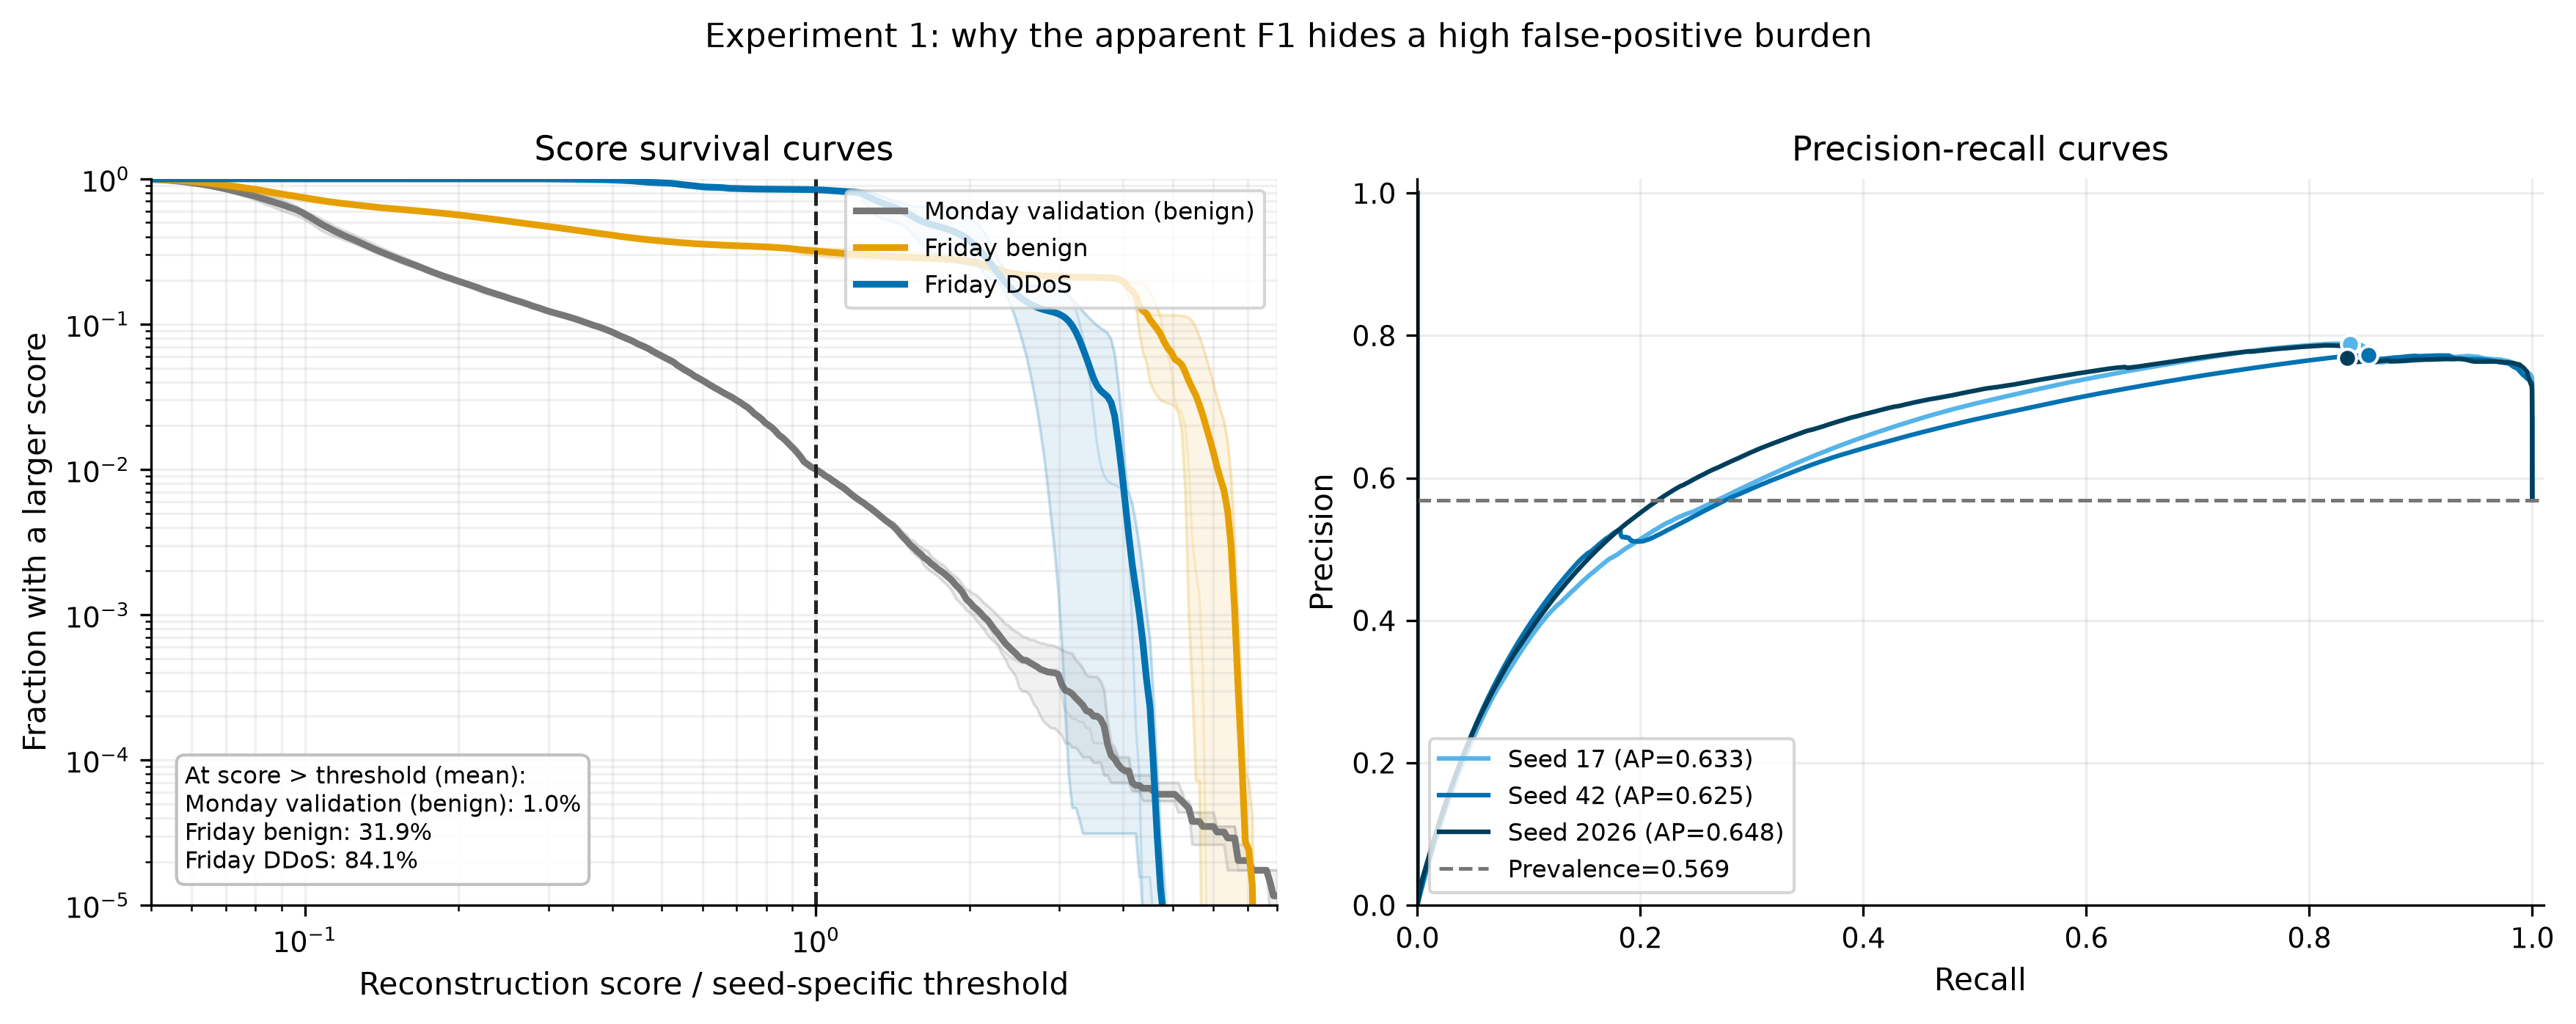
\includegraphics[width=0.95\textwidth]{figures/experiment_01_scores_and_pr.png}
\caption{Normalized reconstruction-score distributions and precision-recall behavior. The threshold calibrated on Monday does not transfer cleanly to benign Friday traffic.}
\label{fig:exp1_scores}
\end{figure}

False positives concentrate in shifted benign subpopulations. For example,
positive URG flags rise from 6.12\% of Monday training flows to 32.61\% of
Friday benign flows. Ports also change in prevalence, although ports and
identifiers were excluded from VAE input.

A threshold-sensitivity analysis confirms that the problem cannot be solved simply by choosing a more conservative threshold. Raising the threshold reduces the Friday false-positive rate only moderately, while recall drops sharply. For example, moving from a 1\% to a 0.1\% target false-positive rate on Monday validation reduces the Friday false-positive rate from 31.92\% to 26.22\%, but recall falls from 84.13\% to 33.93\%.

Thus learning normal traffic nonlinearly does not ensure cross-day calibration.
Experiment 3 reuses these exact scores to test whether destination-time groups
help distinguish attacks from benign changes.

% The following block documents the superseded 50-channel pilot and is excluded
% from the compiled report.  The paper-routed experiment follows after \fi.
\iffalse
\subsection{Experiment 2: Linear-to-Nonlinear Synthetic Traffic}

The second experiment studies a controlled synthetic setting with 50 observed features divided into 10 groups of 5 features. The normal signal is generated from a three-dimensional latent state. A parameter $\alpha \in \{0,0.25,0.5,0.75,1\}$ controls the transition from a purely linear low-rank normal signal to a nonlinear low-dimensional normal signal:
\[
L(\alpha) = (1-\alpha)L_{\mathrm{linear}} + \alpha L_{\mathrm{nonlinear}}.
\]
Sparse attacks are injected as non-overlapping group bursts. Each test seed contains 204 attacked time points out of 2,000 time points, corresponding to a 10.2\% time-level attack prevalence. At the group-time and element levels, the attack prevalence is approximately 1.02\%.

Three methods were compared. The first is a normal-only VAE with latent dimension 3. The second is batch RPCA, which decomposes the observed matrix into low-rank and sparse components. The third is an Online Dynamic Anomalography (OnlineDA) adaptation with identity routing, full observations, rank 3, and causal test-time updates. All methods were evaluated on the same generated data within each seed, and thresholds were calibrated from normal validation scores.

\begin{table}[H]
\centering
\caption{Experiment 2: time-level F1 as nonlinearity increases.}
\begin{tabular}{cccc}
\toprule
$\alpha$ & VAE & RPCA & OnlineDA \\
\midrule
0.00 & 0.9586 & 0.9601 & 0.9563 \\
0.25 & 0.9856 & 0.9697 & 0.8758 \\
0.50 & 0.9848 & 0.6139 & 0.3075 \\
0.75 & 0.9849 & 0.2995 & 0.1859 \\
1.00 & 0.9819 & 0.2007 & 0.1280 \\
\bottomrule
\end{tabular}
\end{table}

\begin{figure}[H]
\centering
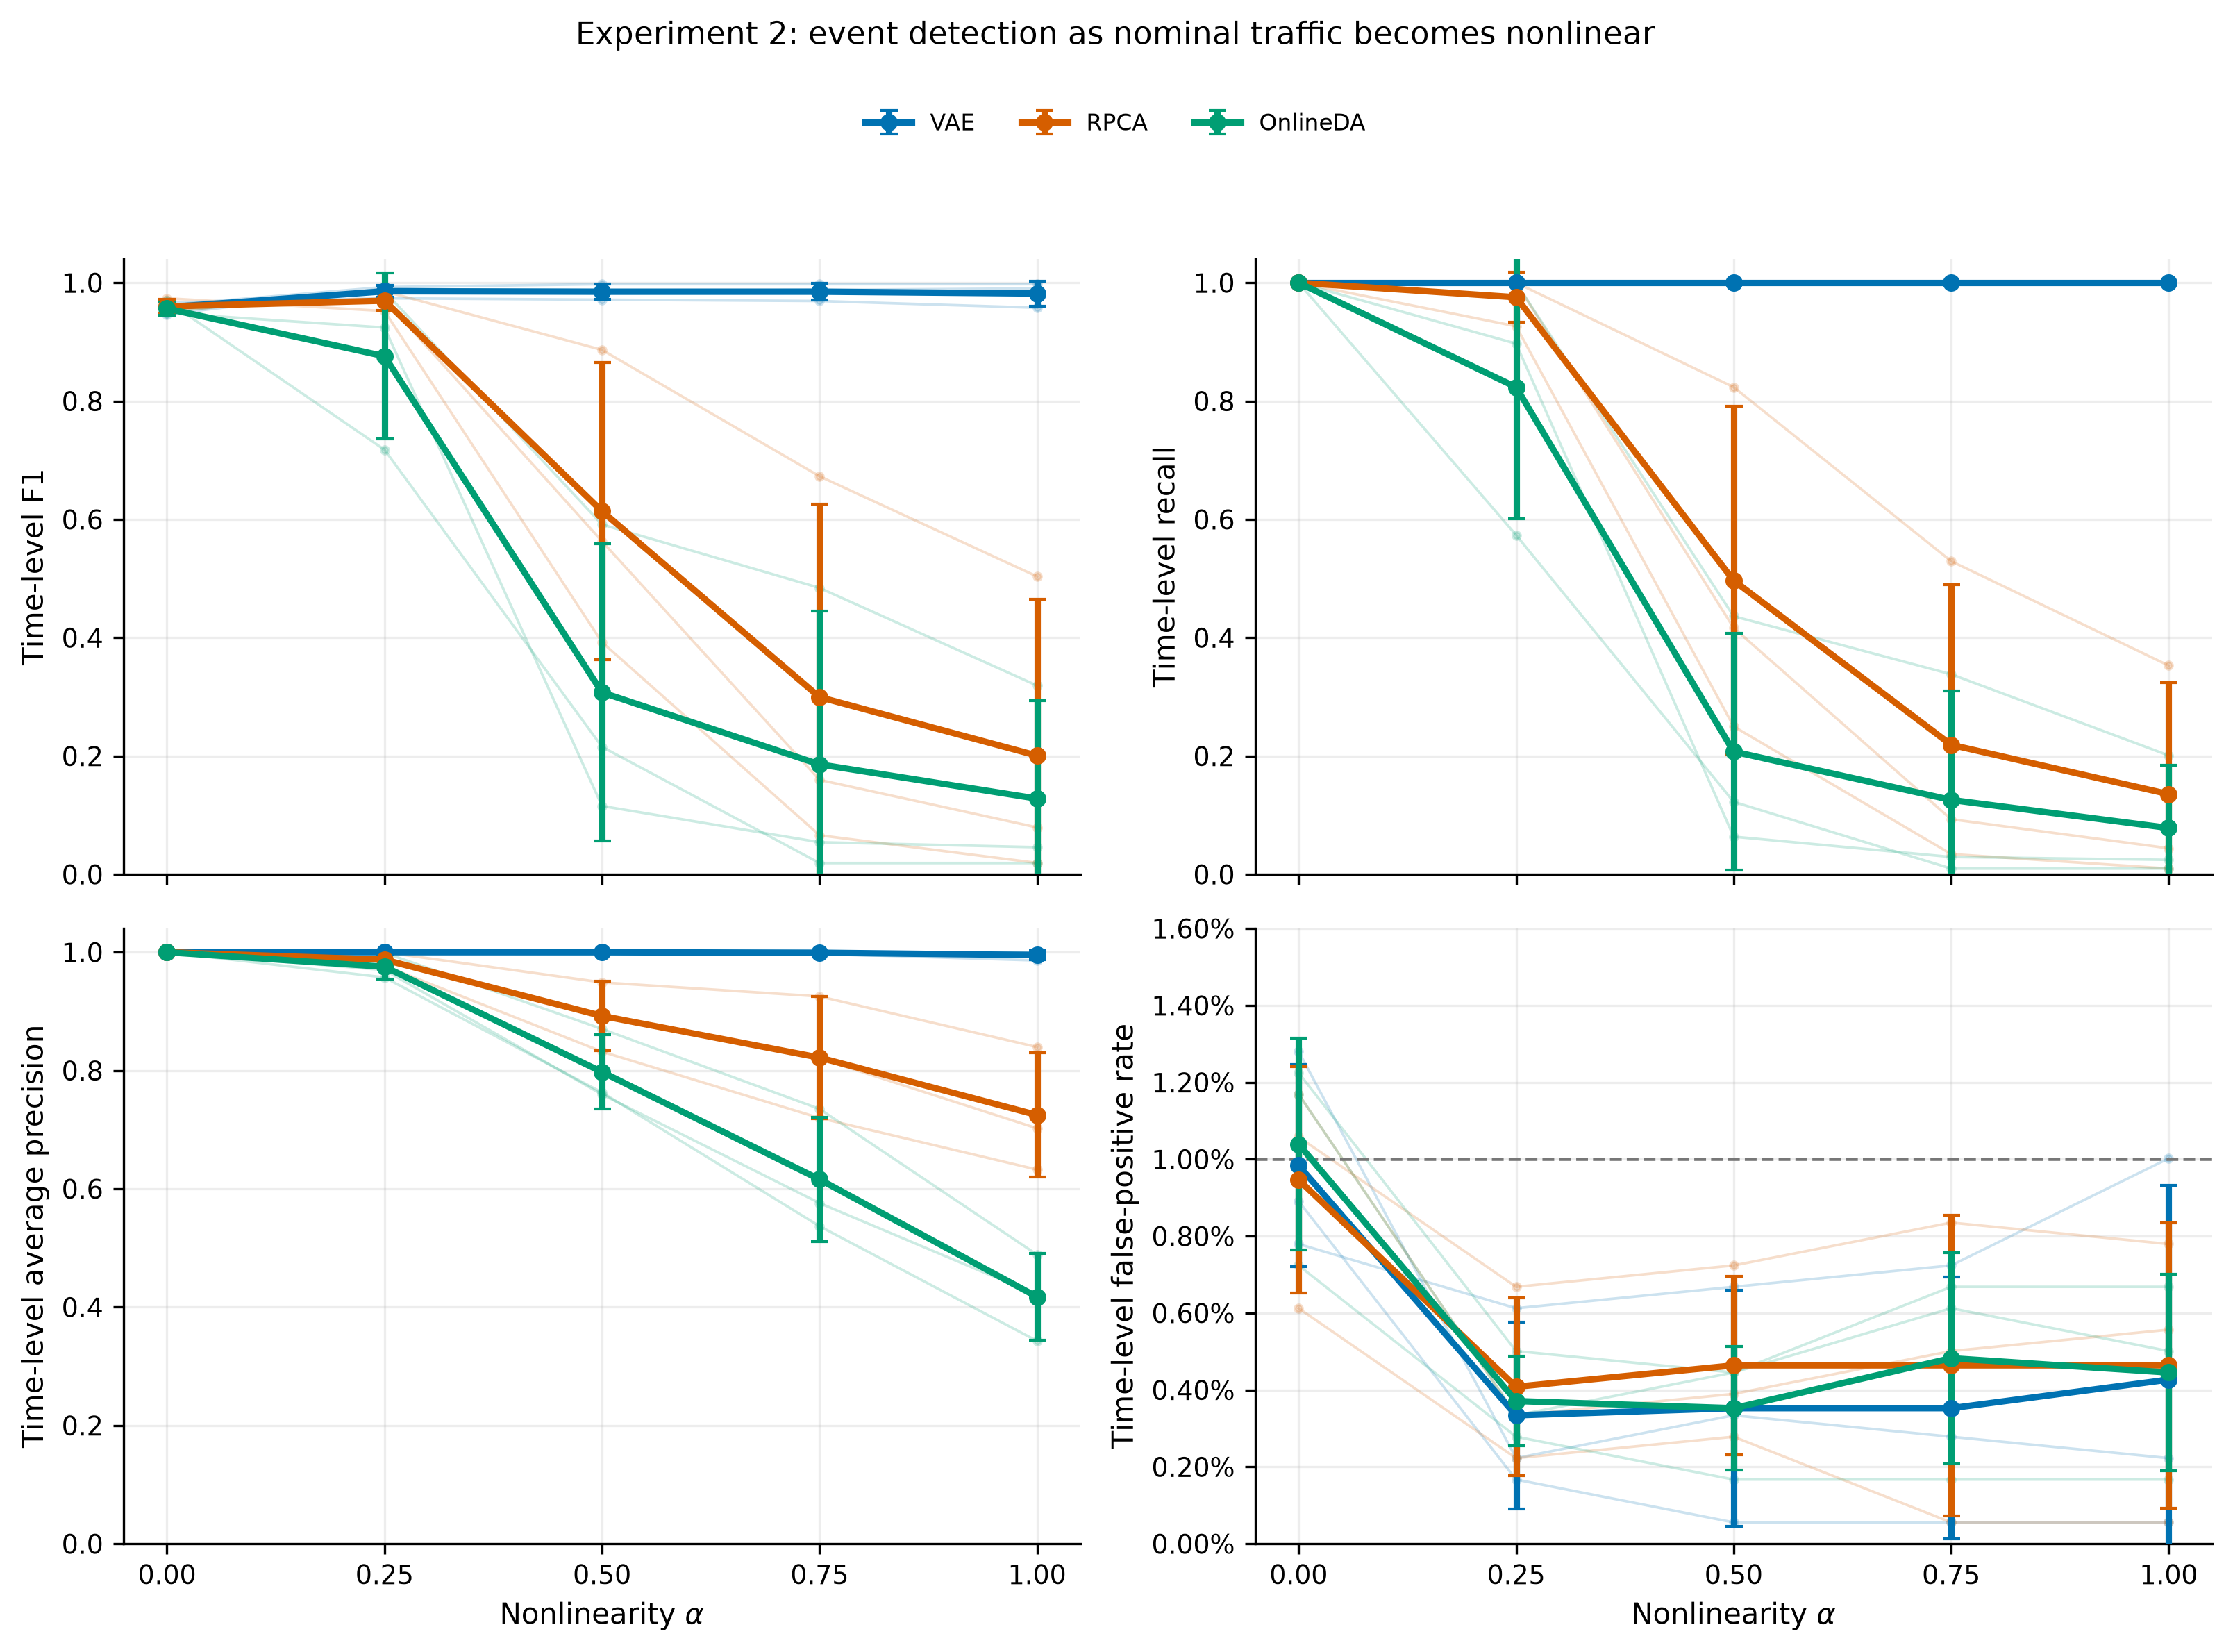
\includegraphics[width=0.95\textwidth]{figures/experiment_02_detection_vs_alpha.png}
\caption{Time-level detection performance as the normal traffic changes from linear to nonlinear.}
\label{fig:exp2_detection}
\end{figure}

At $\alpha=0$, all three methods perform almost identically in time-level detection. This is expected because the normal component is truly low-rank and therefore matches the assumptions of RPCA and OnlineDA. In this linear case, the VAE does not provide a meaningful advantage, and the linear sparse-decomposition methods recover the clean and sparse components more accurately.

As $\alpha$ increases, the behavior changes. Starting from $\alpha=0.5$, the VAE achieves a higher time-level F1 score than both baselines in every seed. At $\alpha=1$, the VAE obtains precision 0.9649, recall 1.0000, false-positive rate 0.0043, and average precision 0.9952. In contrast, RPCA recall drops to 0.1356 and OnlineDA recall drops to 0.0784, while their false-positive rates remain similar to the VAE. Thus, the main failure mode of the linear methods is not an increase in false alarms, but a loss of recall: they miss most attack time points under nonlinear nominal traffic.

\begin{figure}[H]
\centering
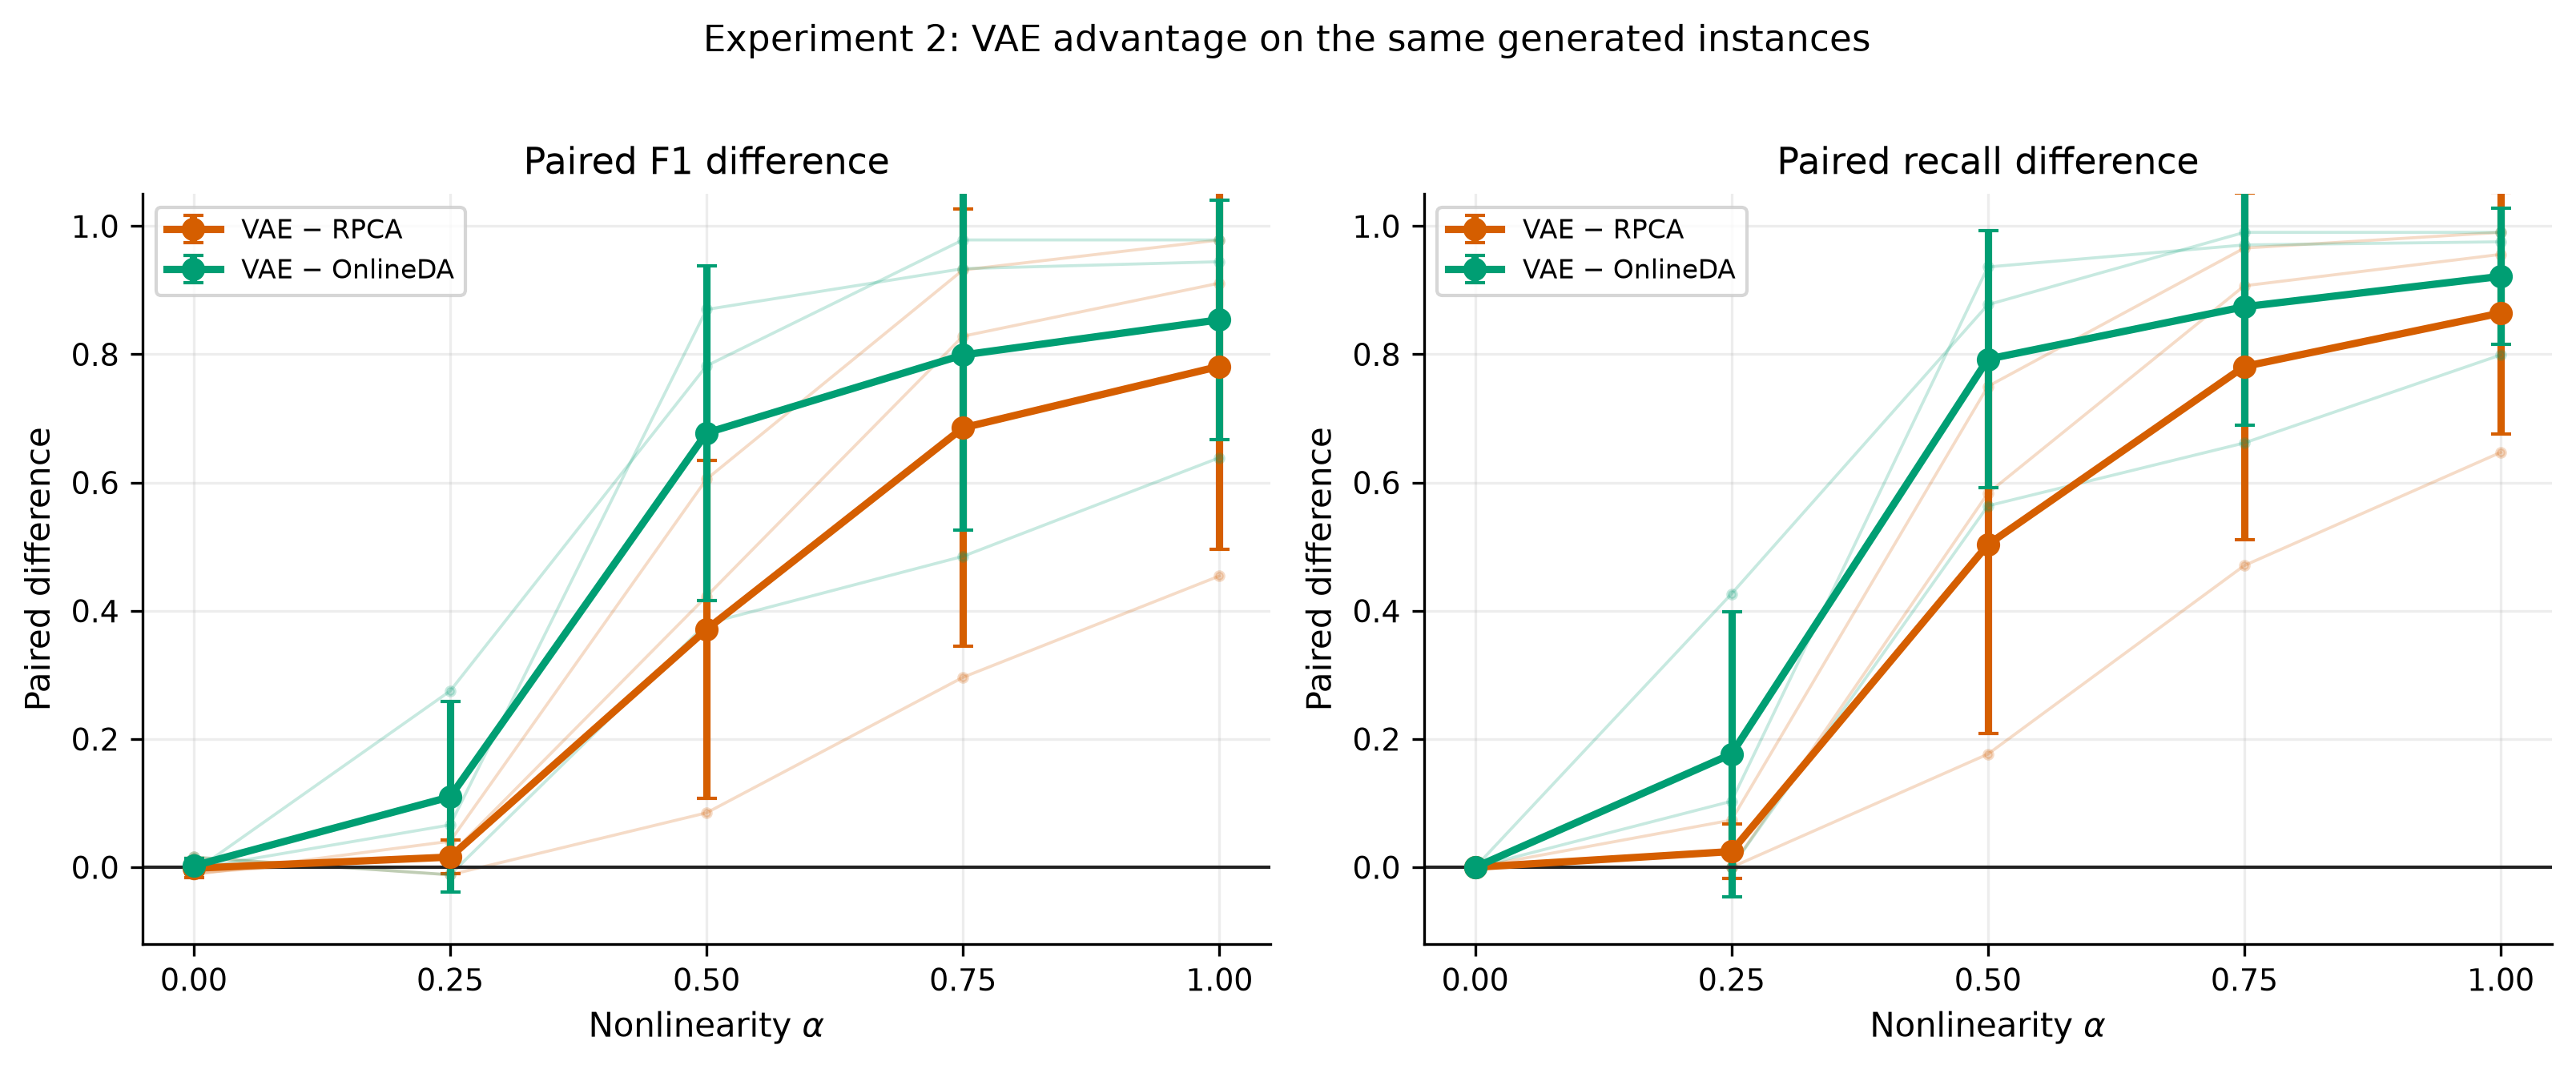
\includegraphics[width=0.95\textwidth]{figures/experiment_02_paired_advantage.png}
\caption{Paired VAE advantage over RPCA and OnlineDA. Values above zero indicate better VAE performance on the same seed and same generated data.}
\label{fig:exp2_paired}
\end{figure}

The mechanism behind this result is visible in the effective rank of the clean signal. Although the latent dimension remains 3 for every value of $\alpha$, the linear rank required to explain the clean signal grows substantially as the generator becomes nonlinear. The mean rank required to explain 99\% of the clean-signal energy increases from 3.00 at $\alpha=0$ to 17.33 at $\alpha=1$. Therefore, the normal traffic remains low-dimensional in a nonlinear sense, but it is no longer well represented by a rank-3 linear subspace. The VAE can model this nonlinear low-dimensional structure, while RPCA and OnlineDA must approximate it using a low-rank linear model.

\begin{table}[H]
\centering
\caption{Experiment 2: recovery errors at the linear and nonlinear endpoints.}
\begin{tabular}{llcc}
\toprule
$\alpha$ & Method & Relative error in $L$ & Relative error in $S$ \\
\midrule
0.00 & VAE & 0.0829 & 0.4664 \\
0.00 & RPCA & 0.0318 & 0.0987 \\
0.00 & OnlineDA & 0.0279 & 0.0948 \\
1.00 & VAE & 0.1285 & 0.6694 \\
1.00 & RPCA & 0.2871 & 1.2081 \\
1.00 & OnlineDA & 0.6468 & 2.8275 \\
\bottomrule
\end{tabular}
\end{table}

\begin{figure}[H]
\centering
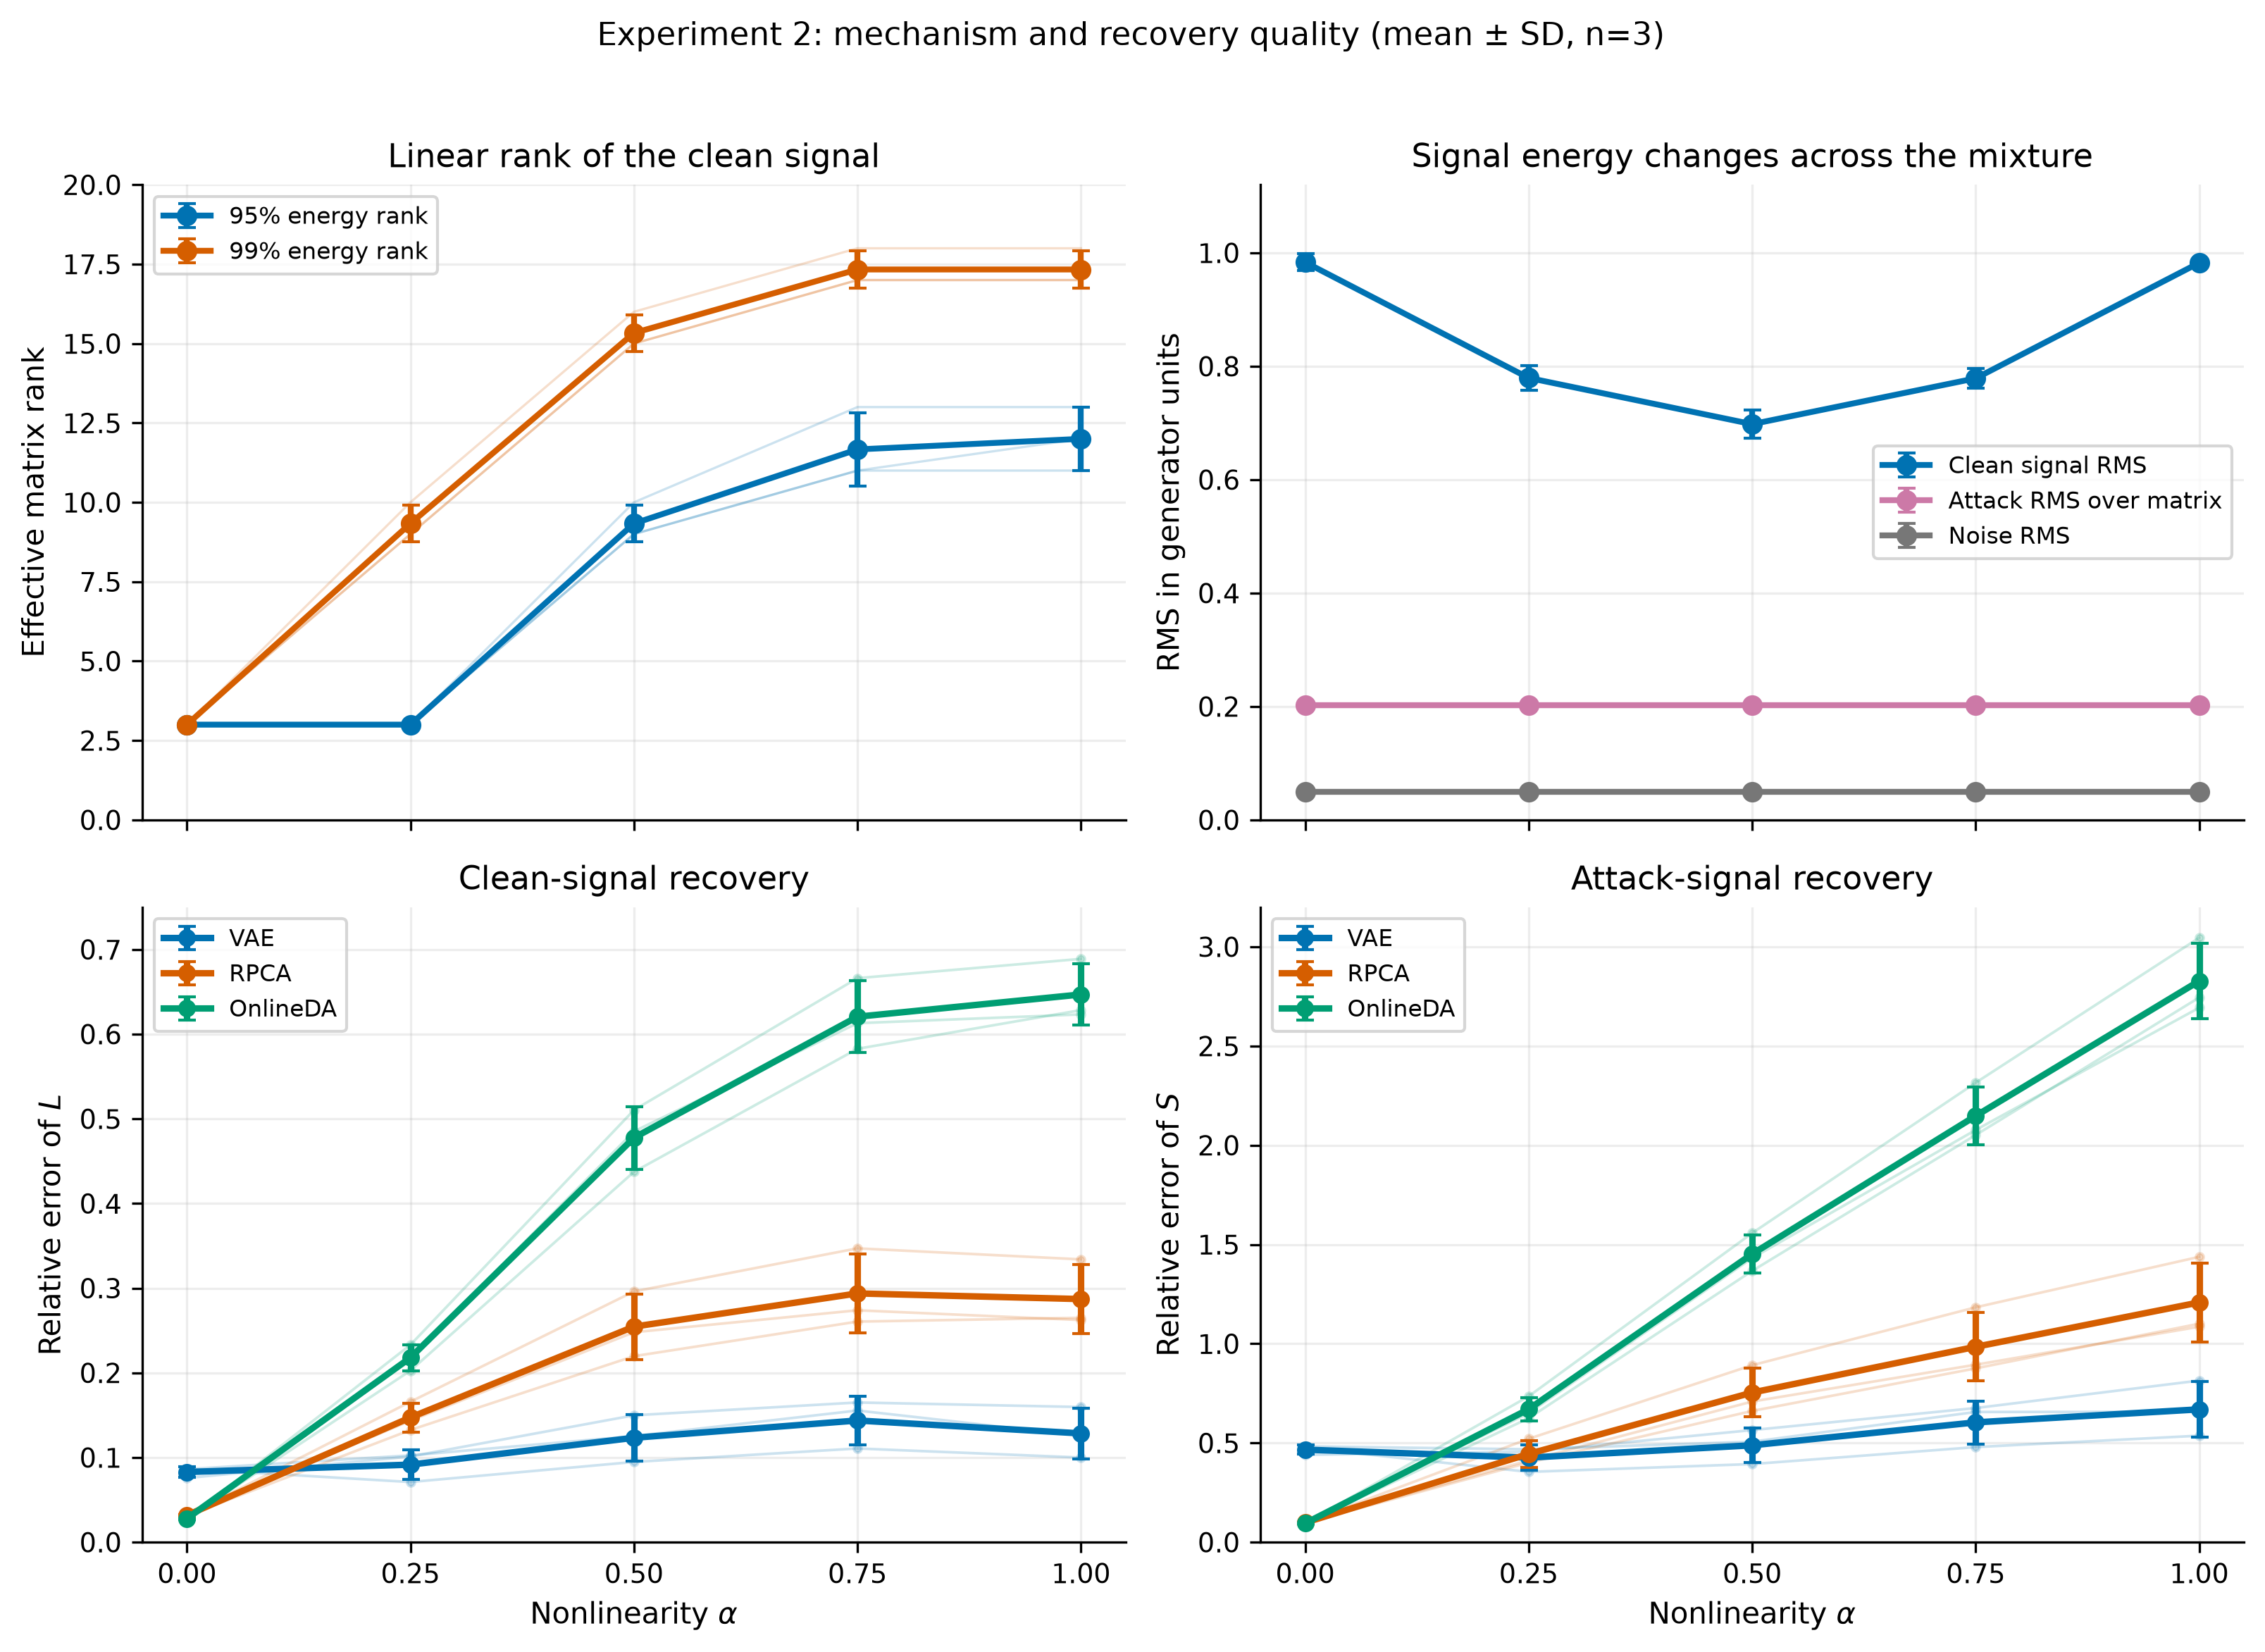
\includegraphics[width=0.95\textwidth]{figures/experiment_02_mechanism_and_recovery.png}
\caption{Effective rank and recovery errors. The VAE becomes favorable when the normal signal is nonlinear but remains low-dimensional.}
\label{fig:exp2_mechanism}
\end{figure}

However, the result is more nuanced at the group-localization level. At $\alpha=1$, the VAE achieves group recall 1.0000 and group average precision 0.9988, indicating that attacked groups are usually ranked highly. Nevertheless, its group F1 is only 0.4275 because the calibrated threshold also selects many benign groups. RPCA obtains group F1 0.7766 and OnlineDA obtains group F1 0.7062 at the same endpoint. Therefore, the VAE is highly effective at detecting \textit{when} an attack occurred, but it is weaker at determining \textit{which group} was attacked under the configured threshold.

\begin{figure}[H]
\centering
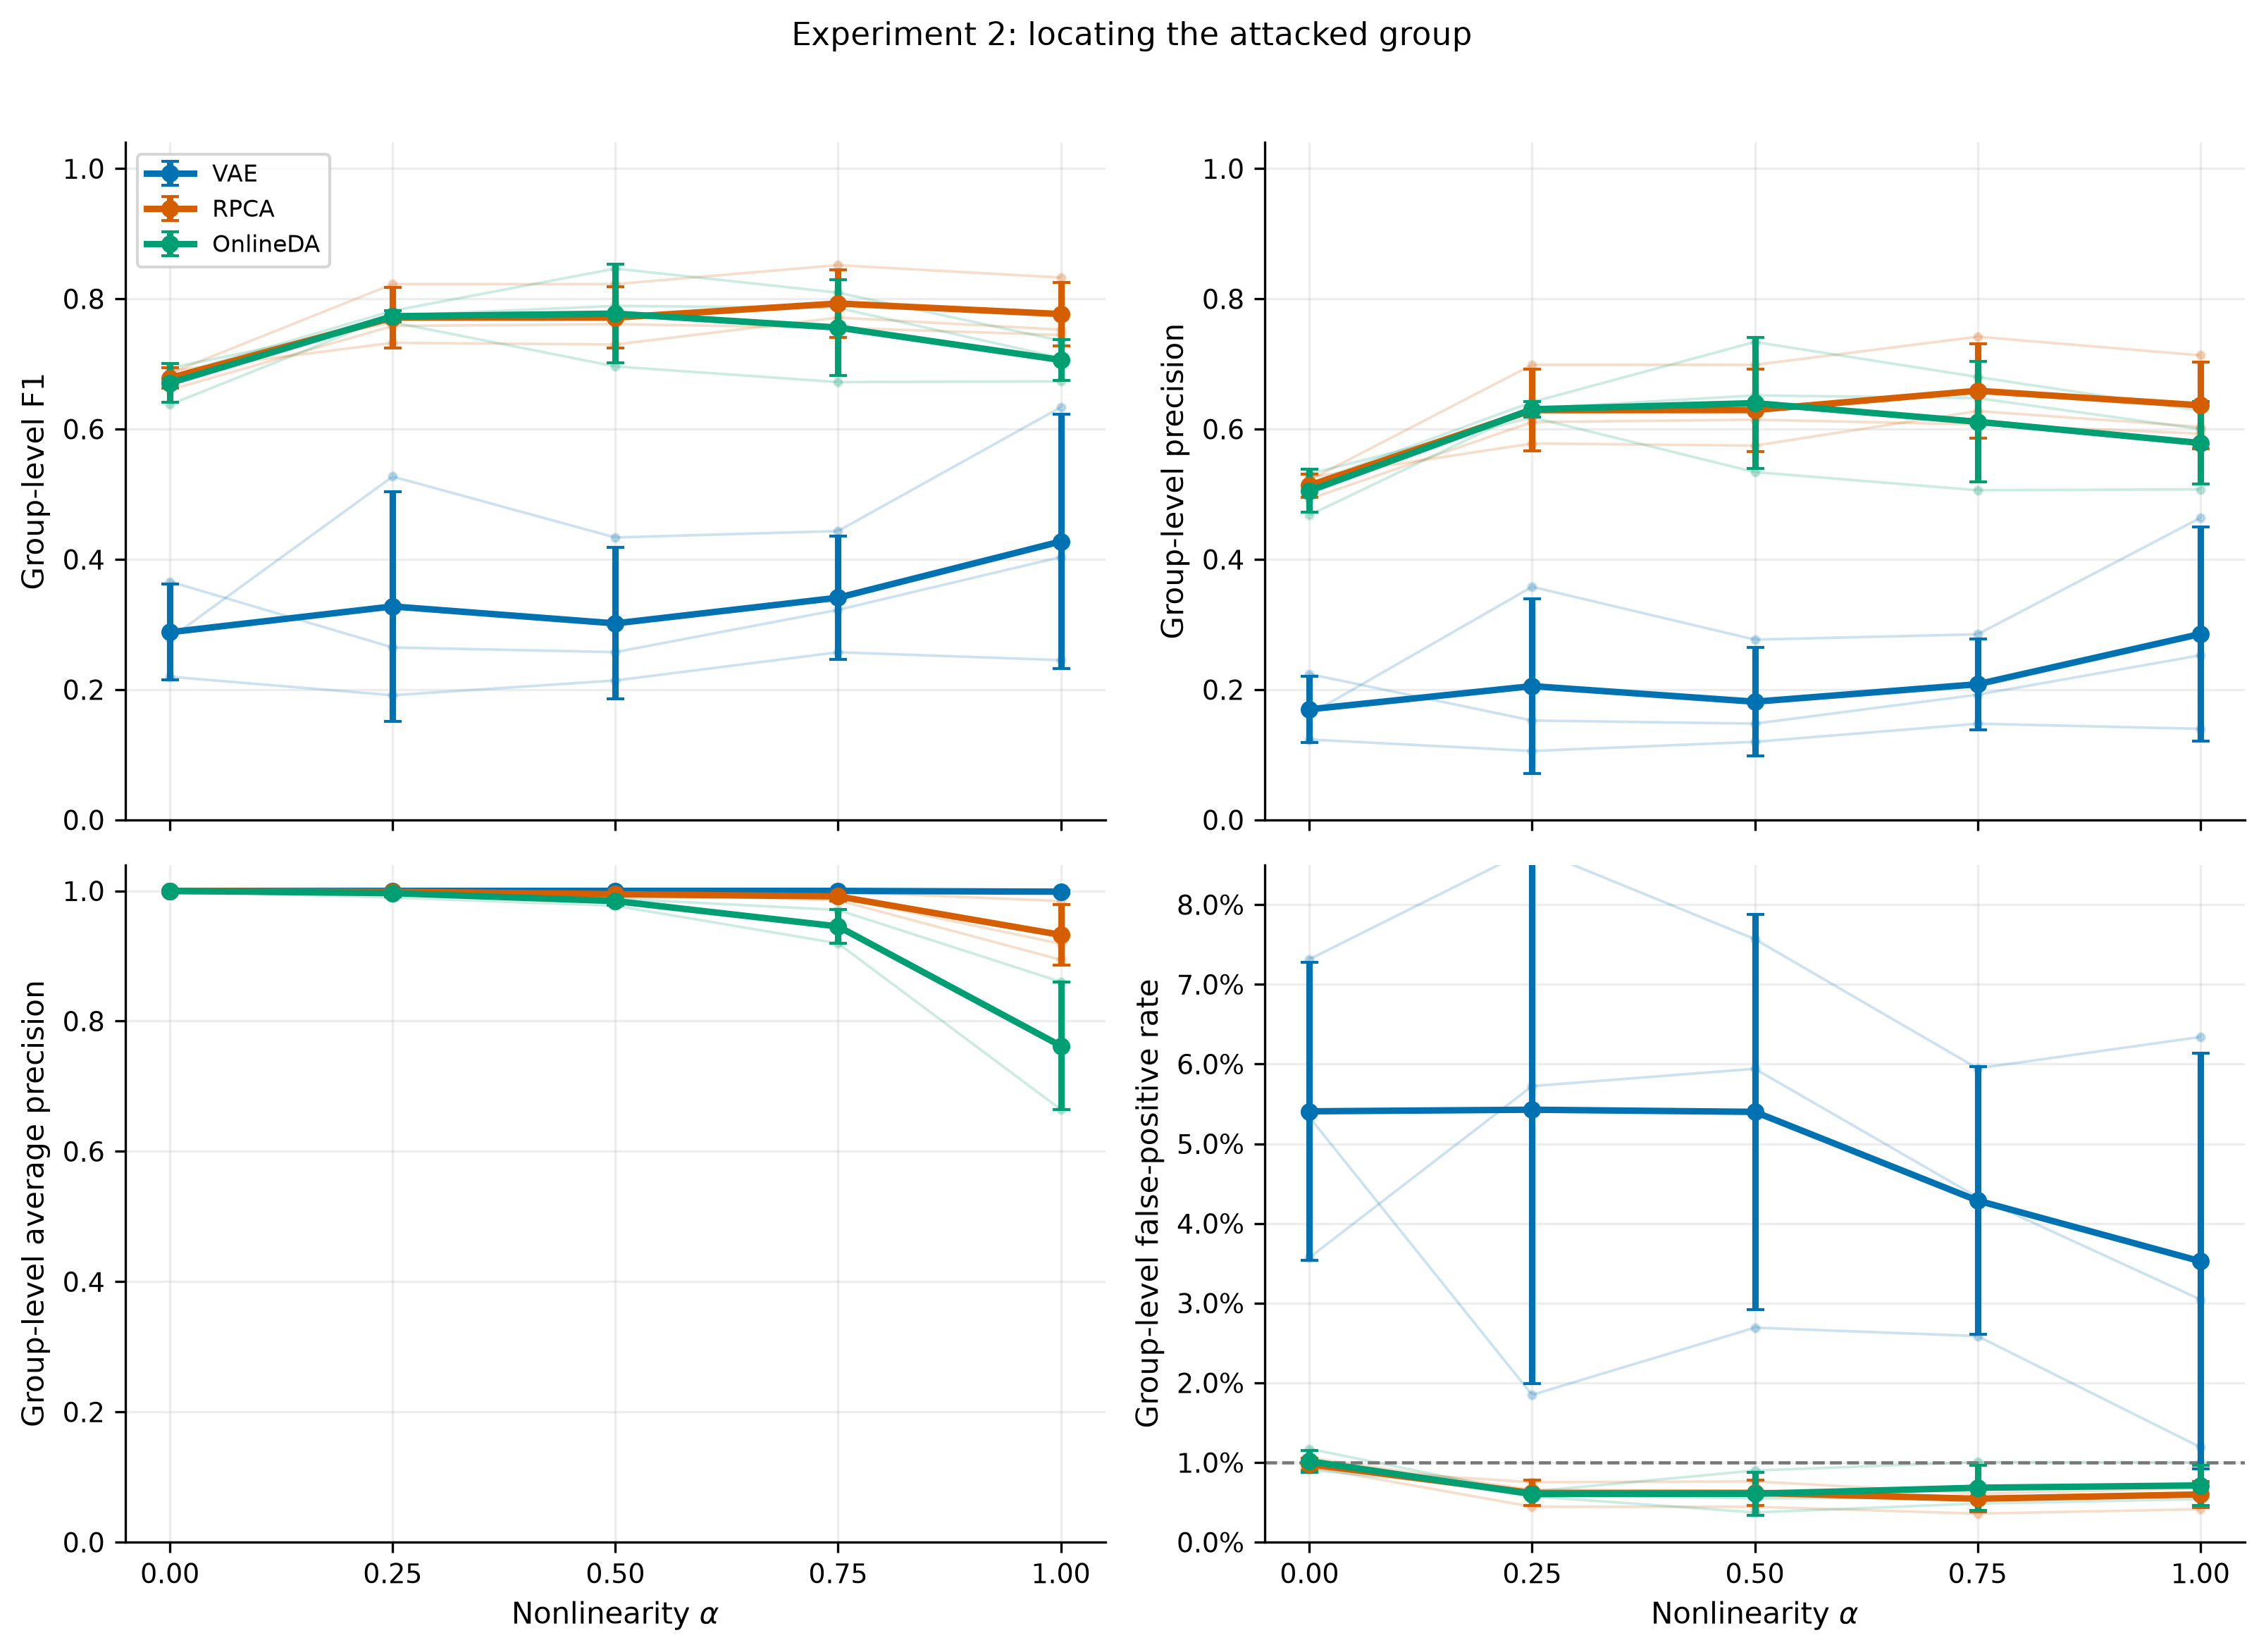
\includegraphics[width=0.95\textwidth]{figures/experiment_02_group_localization.png}
\caption{Group-level localization metrics. Strong time-level detection by the VAE does not automatically imply superior group localization.}
\label{fig:exp2_group}
\end{figure}

The attack-map visualization illustrates the same point qualitatively. In the linear setting, RPCA and OnlineDA produce clean sparse residuals. In the nonlinear setting, the VAE preserves the attack timing well but also produces a denser residual background. This explains why it succeeds in event detection while producing more group-level false positives.

\begin{figure}[H]
\centering
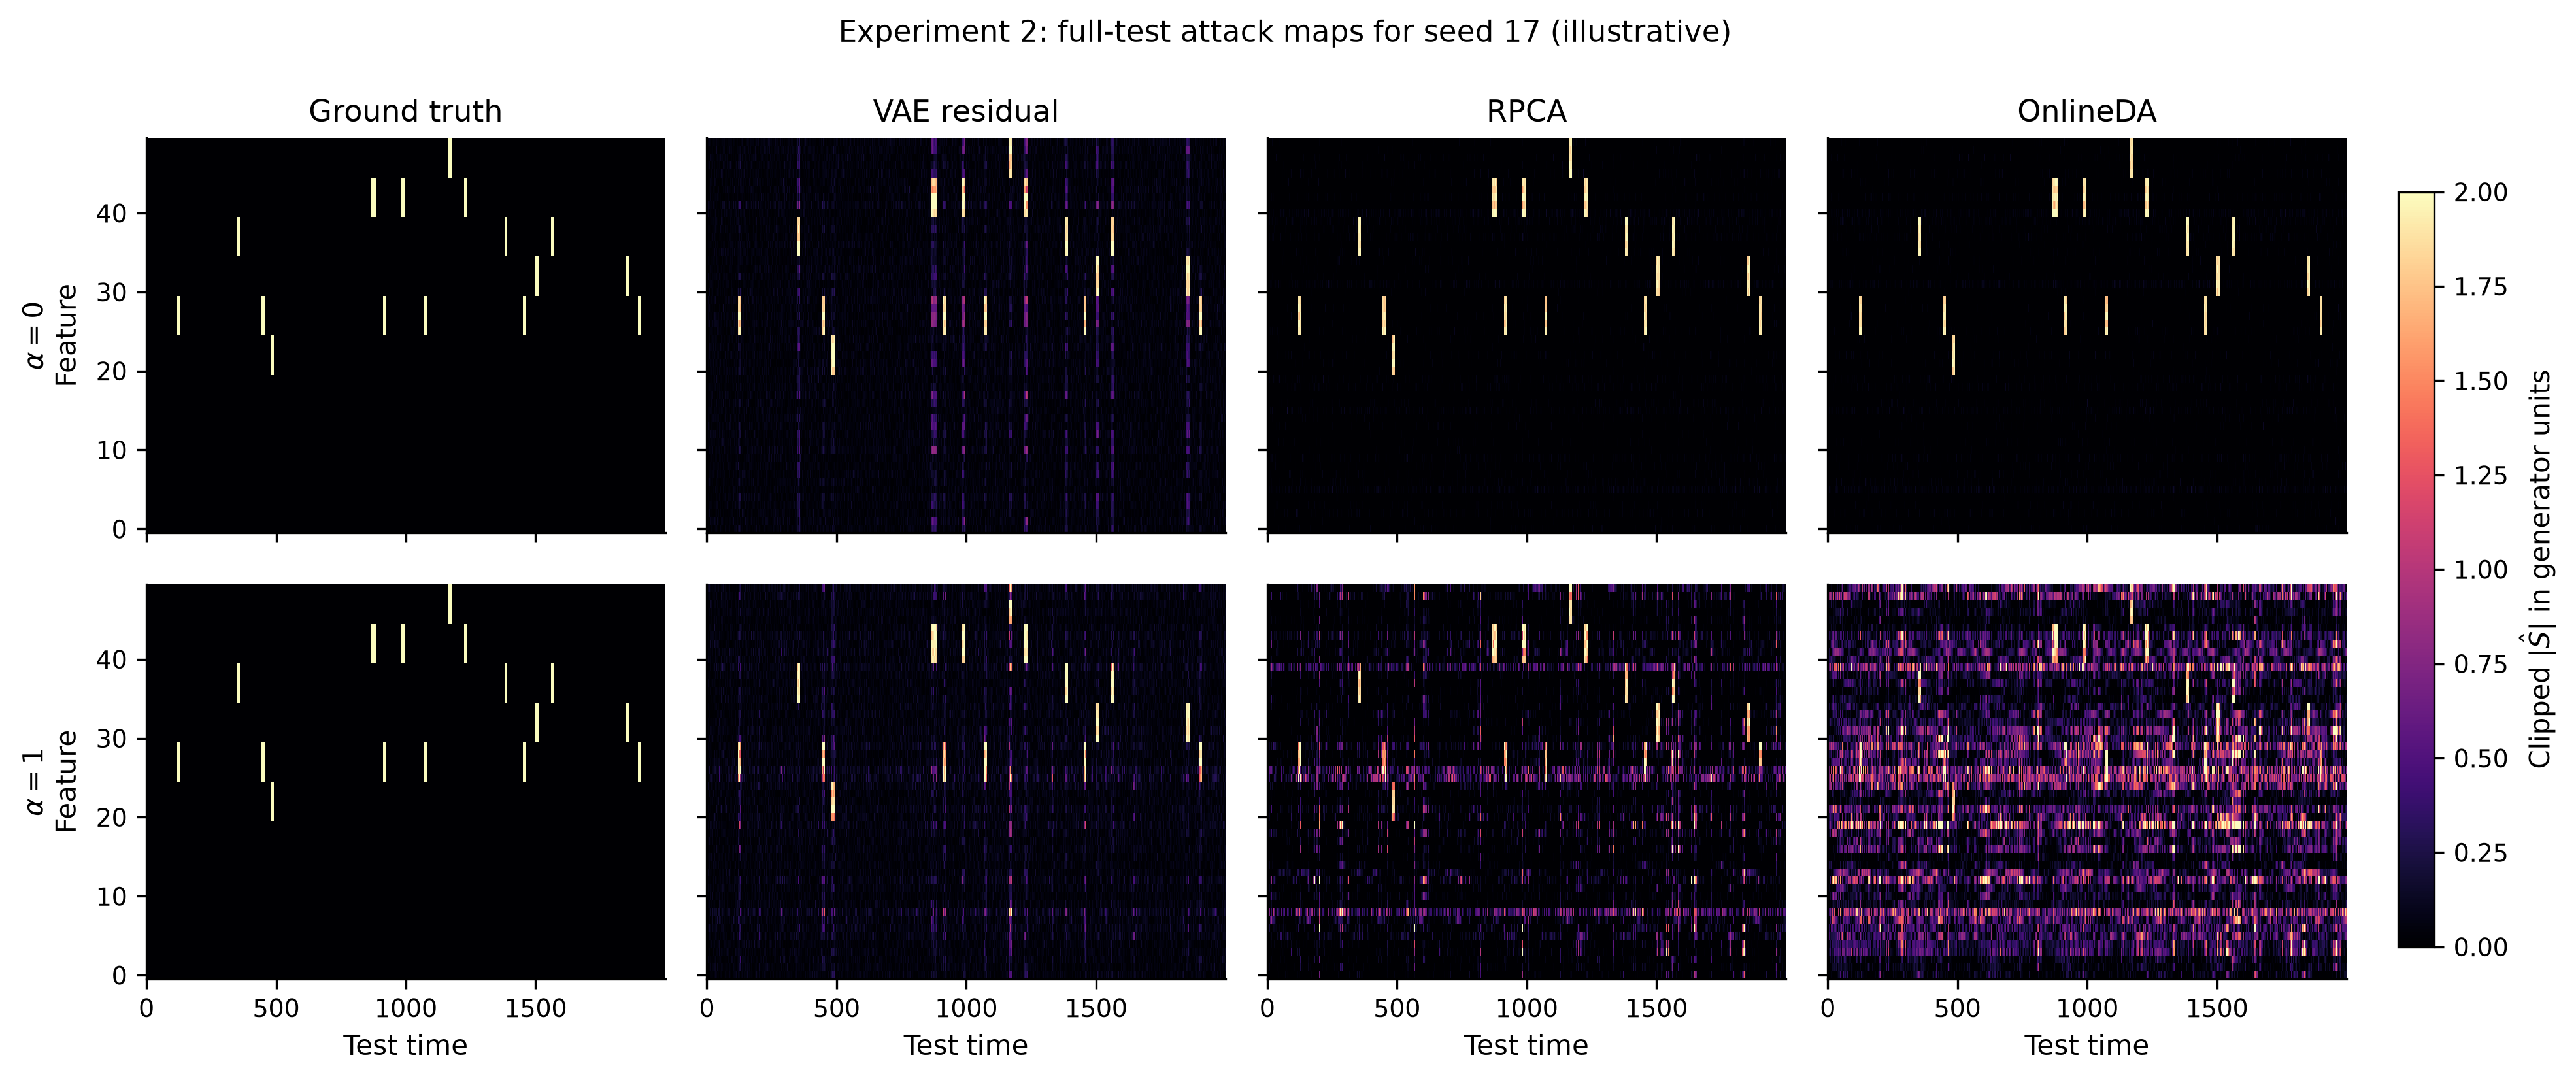
\includegraphics[width=0.95\textwidth]{figures/experiment_02_attack_maps_seed_17.png}
\caption{Example residual maps for one seed. The nonlinear case shows the VAE preserving attack timing but with denser residual noise.}
\label{fig:exp2_maps}
\end{figure}

\fi

\subsection{Experiment 2: Paper-Routed Linear Control and Nonlinear Extension}

The second experiment replaces the earlier identity-routing pilot with the
synthetic network model specified in Section VI-A of Mardani et
al.~\cite{Mardani}.  For each of three fixed seeds, 15 nodes are sampled in the
unit square and connected using the paper's distance threshold of 0.35.  We
retain connected graphs with exactly 52 directed links.  The ordered node pairs
define 210 origin--destination (OD) flows, and minimum-hop paths define the
routing matrix $R\in\{0,1\}^{52\times210}$.

At the linear endpoint, nominal OD traffic has rank two, attacks are independent
sparse signed entries with probability $p=0.005$, and link noise has standard
deviation $\sigma=0.01$:
\[
z_t=Uw_t,\qquad
y_t=R(z_t+a_t)+v_t.
\]
This matches the published dimensions and distributions but not the authors'
unpublished random realization.  The main sweep uses static routing and full
link observations.  It contains 6,000 normal training samples, 2,000 normal
validation samples, 2,000 independent normal calibration samples, and 4,000
test samples with injected attacks per seed.

The paper itself assumes a linear low-rank nominal component.  Our extension
introduces a separate nonlinearity parameter $\gamma$ while reserving $\alpha$
for the paper's routing-change probability.  Independent nonlinear maps produce
$G(w_t)$, their routed training energy is matched to the linear endpoint, and
\[
z_t(\gamma)=(1-\gamma)Uw_t+\gamma G(w_t),
\qquad \gamma\in\{0,.25,.5,.75,1\}.
\]
The topology, latent draws, attacks, and noise are paired across $\gamma$ within
each seed.

Two methods are compared.  \textit{VAE+Lasso} trains a two-dimensional VAE only
on normal 52-dimensional link measurements.  The VAE therefore learns nominal
traffic, not attacks.  At test time the OD attack estimate is obtained from the
unexplained link residual using
\[
\hat a_t=\arg\min_a\frac12\|y_t-\hat \ell_t-Ra\|_2^2
                   +0.11\|a\|_1.
\]
\textit{OnlineDA} implements the paper's Algorithm 2 with routing matrix $R$,
rank bound 5, ridge parameter 0.36, sparse penalty 0.11, and a normal-prefix SVD
initialization.  This initialization and the separate normal splits are explicit
adaptations needed for a matched comparison with a frozen VAE.

\begin{table}[H]
\centering
\caption{Experiment 2: mean attack-time and OD-flow F1 across three seeds.}
\begin{tabular}{ccccc}
\toprule
$\gamma$ & VAE time F1 & OnlineDA time F1 & VAE flow F1 & OnlineDA flow F1 \\
\midrule
0.00 & 0.9995 & 0.9942 & 0.1261 & 0.5539 \\
0.25 & 0.9965 & 0.9972 & 0.1314 & 0.4107 \\
0.50 & 0.9962 & 0.9965 & 0.1106 & 0.4031 \\
0.75 & 0.9966 & 0.9964 & 0.1147 & 0.4154 \\
1.00 & 0.9976 & 0.9960 & 0.1391 & 0.4163 \\
\bottomrule
\end{tabular}
\end{table}

Both methods detect almost every attacked time point, so time-level F1 is not
discriminative in this generator.  OD-flow localization gives the important
result: OnlineDA has substantially higher F1 for every $\gamma$.  At $\gamma=1$,
flow average precision is 0.8680 for VAE+Lasso and 0.9295 for OnlineDA, while
flow false-positive rates are 0.0585 and 0.0131, respectively.

\begin{figure}[H]
\centering
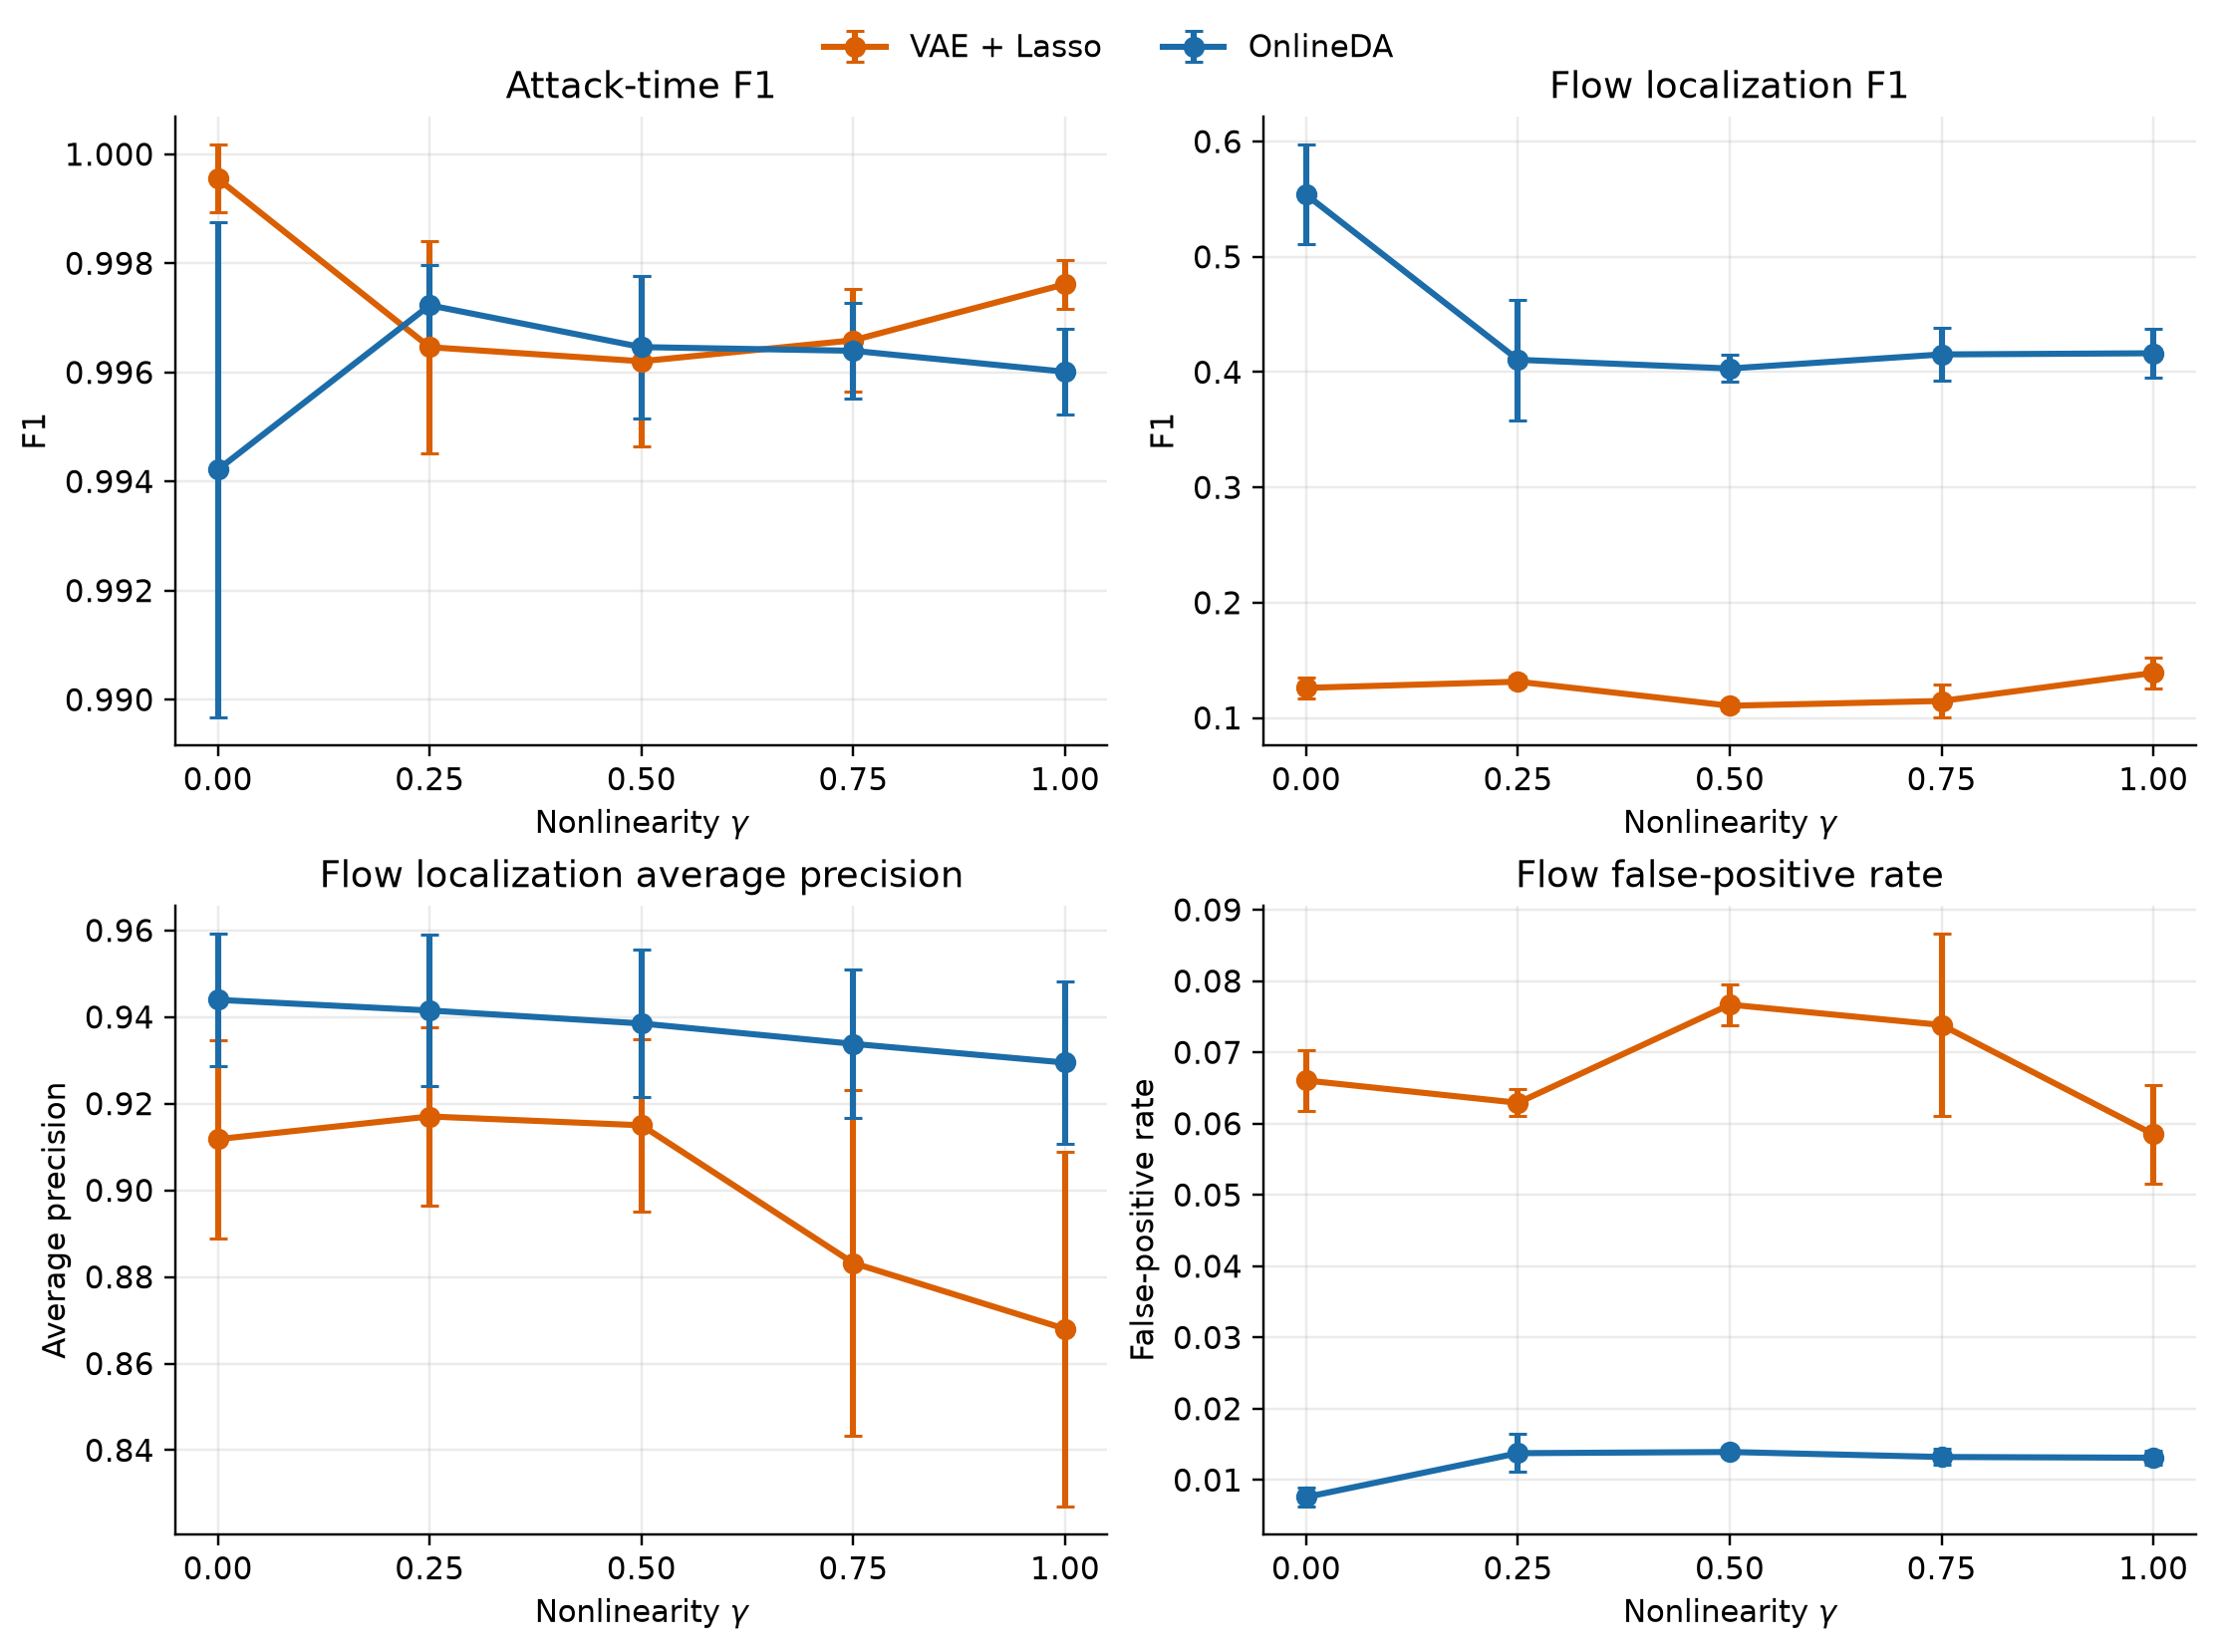
\includegraphics[width=0.98\textwidth]{figures/experiment_02_paper_detection.png}
\caption{Detection and OD-flow localization in the paper-routed nonlinear sweep.
The VAE preserves attack timing but produces a much denser flow residual.}
\label{fig:exp2_paper_detection}
\end{figure}

The nonlinear extension does change the geometry as intended: the mean linear
rank required for 99\% of nominal-link energy rises from 2 at $\gamma=0$ to 9.33
at $\gamma=1$.  Nevertheless, the current VAE does not convert that modeling
capacity into better attack localization.  The inverse problem has only 52 link
measurements for 210 OD-flow coefficients, so dense reconstruction error is
amplified by sparse decoding.  At $\gamma=1$, relative OD-anomaly recovery error
is 0.5860 for VAE+Lasso and 0.4276 for OnlineDA.

\begin{figure}[H]
\centering
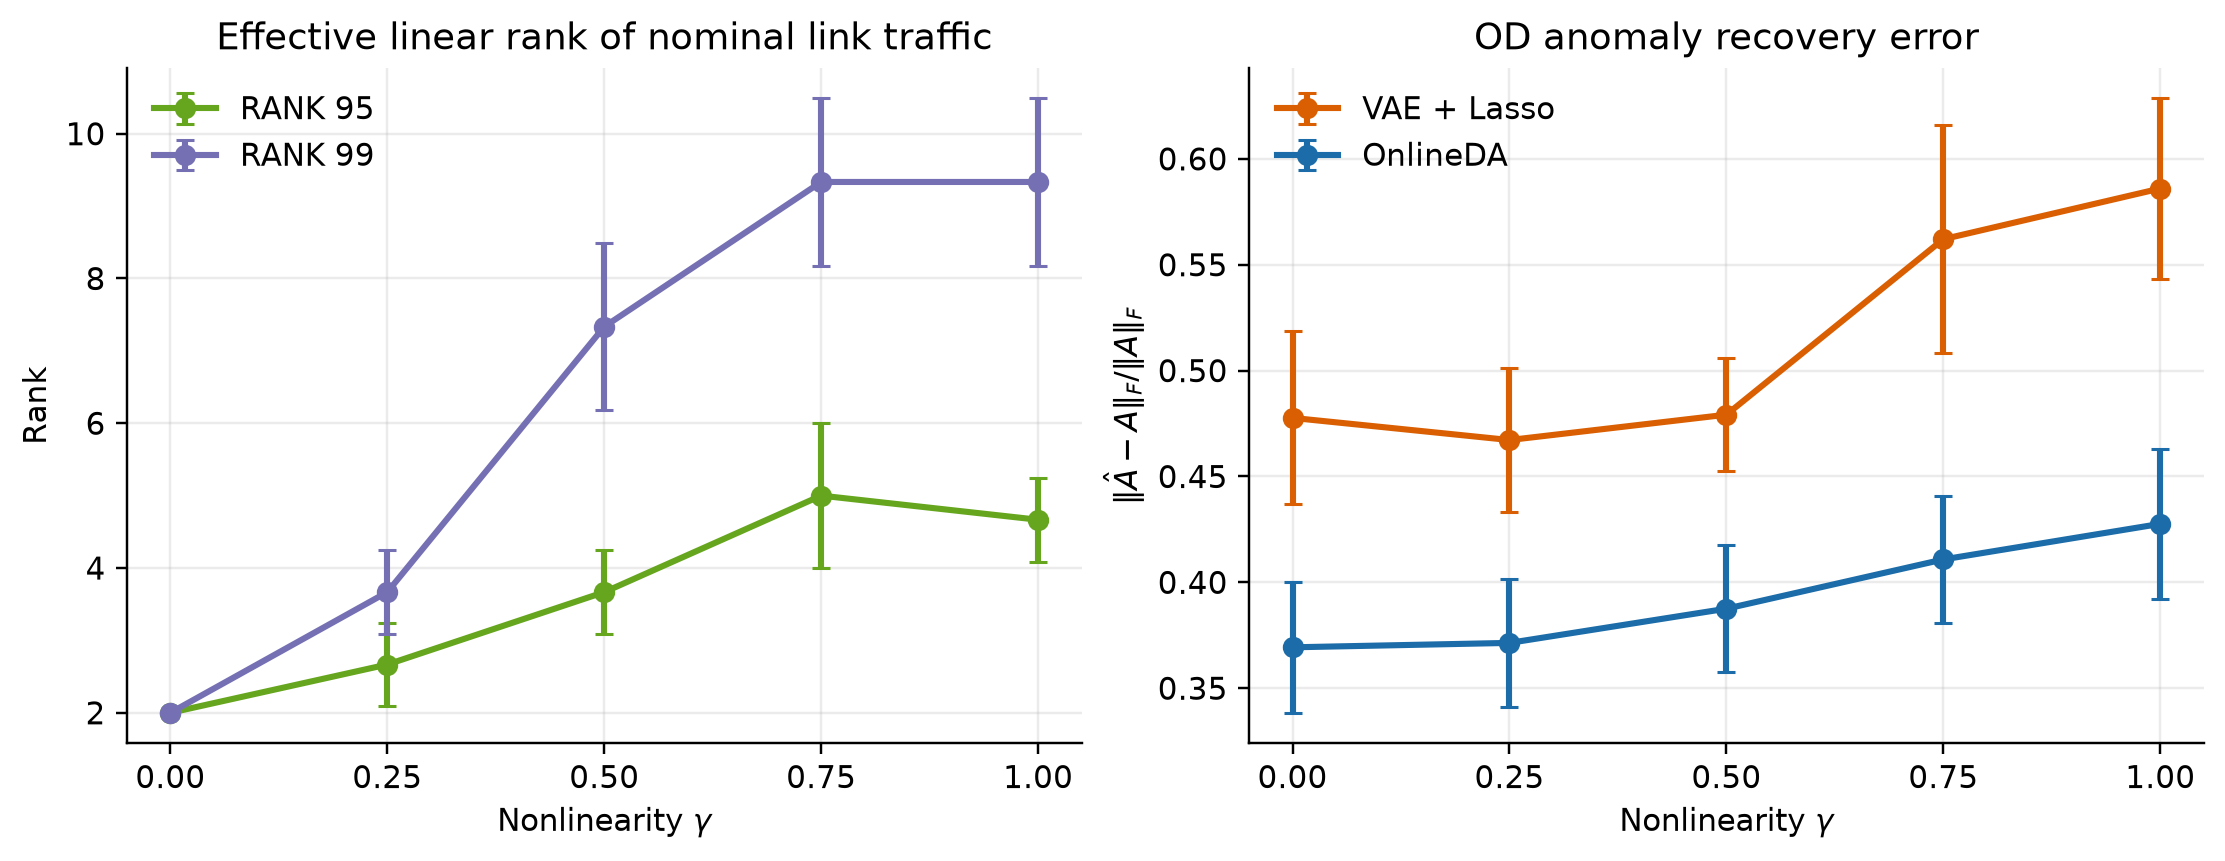
\includegraphics[width=0.98\textwidth]{figures/experiment_02_paper_rank_recovery.png}
\caption{The effective linear rank grows with $\gamma$, but the configured VAE
still has higher OD-anomaly recovery error.}
\label{fig:exp2_paper_rank}
\end{figure}

Following the parameter combinations around Figure 4 of the paper, a separate
linear-endpoint stress suite uses forgetting factor $\beta=0.9$, 1,000-sample
test streams, time-varying routing, and missing link measurements.  The four
parameter triples $(\alpha,\pi,\sigma)$ are
\[
(.01,.8,.01),\quad (.01,.8,10^{-5}),\quad
(.1,.8,10^{-5}),\quad (.01,1,10^{-5}).
\]

\begin{table}[H]
\centering
\caption{Paper-style tracking stress tests: mean flow F1 / average precision.}
\begin{tabular}{ccc}
\toprule
$(\alpha,\pi,\sigma)$ & VAE+Lasso & OnlineDA \\
\midrule
$(.01,.8,.01)$ & 0.2217 / 0.3793 & 0.2335 / 0.3810 \\
$(.01,.8,10^{-5})$ & 0.2213 / 0.3832 & 0.2342 / 0.3819 \\
$(.1,.8,10^{-5})$ & 0.2790 / 0.3480 & 0.2748 / 0.3332 \\
$(.01,1,10^{-5})$ & 0.3002 / 0.7560 & 0.3535 / 0.7977 \\
\bottomrule
\end{tabular}
\end{table}

There is no stable winner under tracking stress: OnlineDA has higher flow F1 in
three scenarios, whereas VAE+Lasso is slightly higher under rapid routing
changes.  Both deteriorate strongly relative to static routing.  The VAE models
raw link observations and is not conditioned explicitly on $R_t$ or the missing
data mask, which limits invariance to topology and observation changes.

The reference objective uses elementwise $\|A\|_1$ and independent attacks, not
Group Lasso. This baseline is retained unchanged; destination-grouped decoding
and matched structured attacks are introduced separately in Experiment 3.

Finally, the article's real Internet2 experiment cannot be reproduced exactly
from the publication alone.  The authors' traffic files, topology snapshot,
observation masks, pseudo-ground-truth output, and random seed are not distributed
with the paper.  Substituting another Internet2/Abilene archive would be a new
experiment and is therefore not presented as a reproduction here.

\subsection{Experiment 3: VAE with Ordinary versus Grouped Sparse Decoding}

This extension directly tests the proposed combination of a nonlinear normal
model and a group-sparsity optimization stage. The two VAE decoders reuse the
same frozen model within each seed and setting; no additional VAE is trained.
OnlineDA is a third baseline in the synthetic arm only. The
seeds remain 17, 42, and 2026. Two complementary arms use the recorded flows
from Experiment 1 and the routed synthetic network from Experiment 2. They
answer different questions and are not presented as the same inverse problem.

\subsubsection{Recorded CICIDS2017 flows: destination-time score denoising}

The CICIDS2017 capture supplies flow labels, destination IPs, and timestamps
\cite{CICIDS2017}. We reuse exactly the 114,806 Monday validation scores and
225,104 Friday test scores from Experiment 1, checking CSV hashes and row IDs.
Groups contain flows to the same destination in a fixed 60-second wall-clock
window. Labels do not determine groups; IPs and timestamps remain excluded from
VAE inputs. Windows are evaluated after completion, so this is an offline
procedure rather than an immediate per-flow alarm.

There is no measured link-to-OD routing matrix in these flow CSVs. We therefore
test an explicitly limited \emph{score-denoising} model, not physical OD attack
recovery. Let $s_i$ be the original VAE reconstruction norm. The alternatives are
\[
 \min_b\frac12\|s-b\|_2^2+\lambda\mathcal R(b),\qquad
 \mathcal R(b)=\|b\|_1\quad\hbox{or}\quad
 \sum_g\sqrt{|G_g|}\,\|b_{G_g}\|_2.
\]
The group penalty follows the size-weighted Group-Lasso construction
\cite{YuanLin2006}. With identity design, the solutions are exact soft
thresholding and block soft thresholding. In particular,
\[
 \hat b_{G_g}=\left(1-\frac{\lambda\sqrt{|G_g|}}
 {\|s_{G_g}\|_2}\right)_+s_{G_g},
\]
with zero output for a zero-norm block. These outputs are anomaly scores,
not attack-volume estimates. The primary $\lambda$ is the normal-score median
for each VAE. Multipliers $0.5,1,2$ are reported as a fixed sensitivity grid;
the primary multiplier remains 1, without selection on test labels.

Each method uses its normal-score 99th percentile as the flow threshold.
Group scores are block root-mean-square values, calibrated on normal groups;
a group is positive when it contains at least one labeled attack. As in
Experiment 1, Monday validation was also used for VAE early stopping, so this
arm has no independently reserved calibration split. There are 8,349 test
groups, only 22 of which contain attacks. All 22 also contain benign flows.
The median group size is 2, the maximum is 8,252, and 42.1\% are singletons.

\begin{table}[H]
\centering
\caption{Experiment 3 on recorded flows: primary-setting means across three
frozen VAE seeds. FPR refers to benign Friday flows.}
\begin{tabular}{lcc}
\toprule
Metric & VAE+Lasso & VAE+Group Lasso \\
\midrule
Flow precision & 0.7767 & 0.7715 \\
Flow recall & 0.8413 & 0.8477 \\
Flow F1 & 0.8076 & 0.8078 \\
Flow FPR & 0.3192 & 0.3312 \\
Flow average precision & 0.6353 & 0.6349 \\
Group F1 & 0.2386 & 0.2386 \\
Group average precision & 0.1700 & 0.1690 \\
\bottomrule
\end{tabular}
\label{tab:exp3_real}
\end{table}

The F1 difference is only 0.0002, while FPR increases by about 1.20 percentage
points. Across the sensitivity grid, the largest mean F1 gain is below 0.0011
and flow average precision does not improve. Ordinary score soft thresholding
leaves the calibrated flow decisions unchanged here, explaining its agreement
with the plain VAE baseline. For the grouped identity model, block RMS is
itself merely soft thresholded; group rankings therefore do not acquire new
information. This sanity check does not demonstrate an effective learned
group-aware traffic model or removal of cross-day distribution shift.

\begin{figure}[H]
\centering
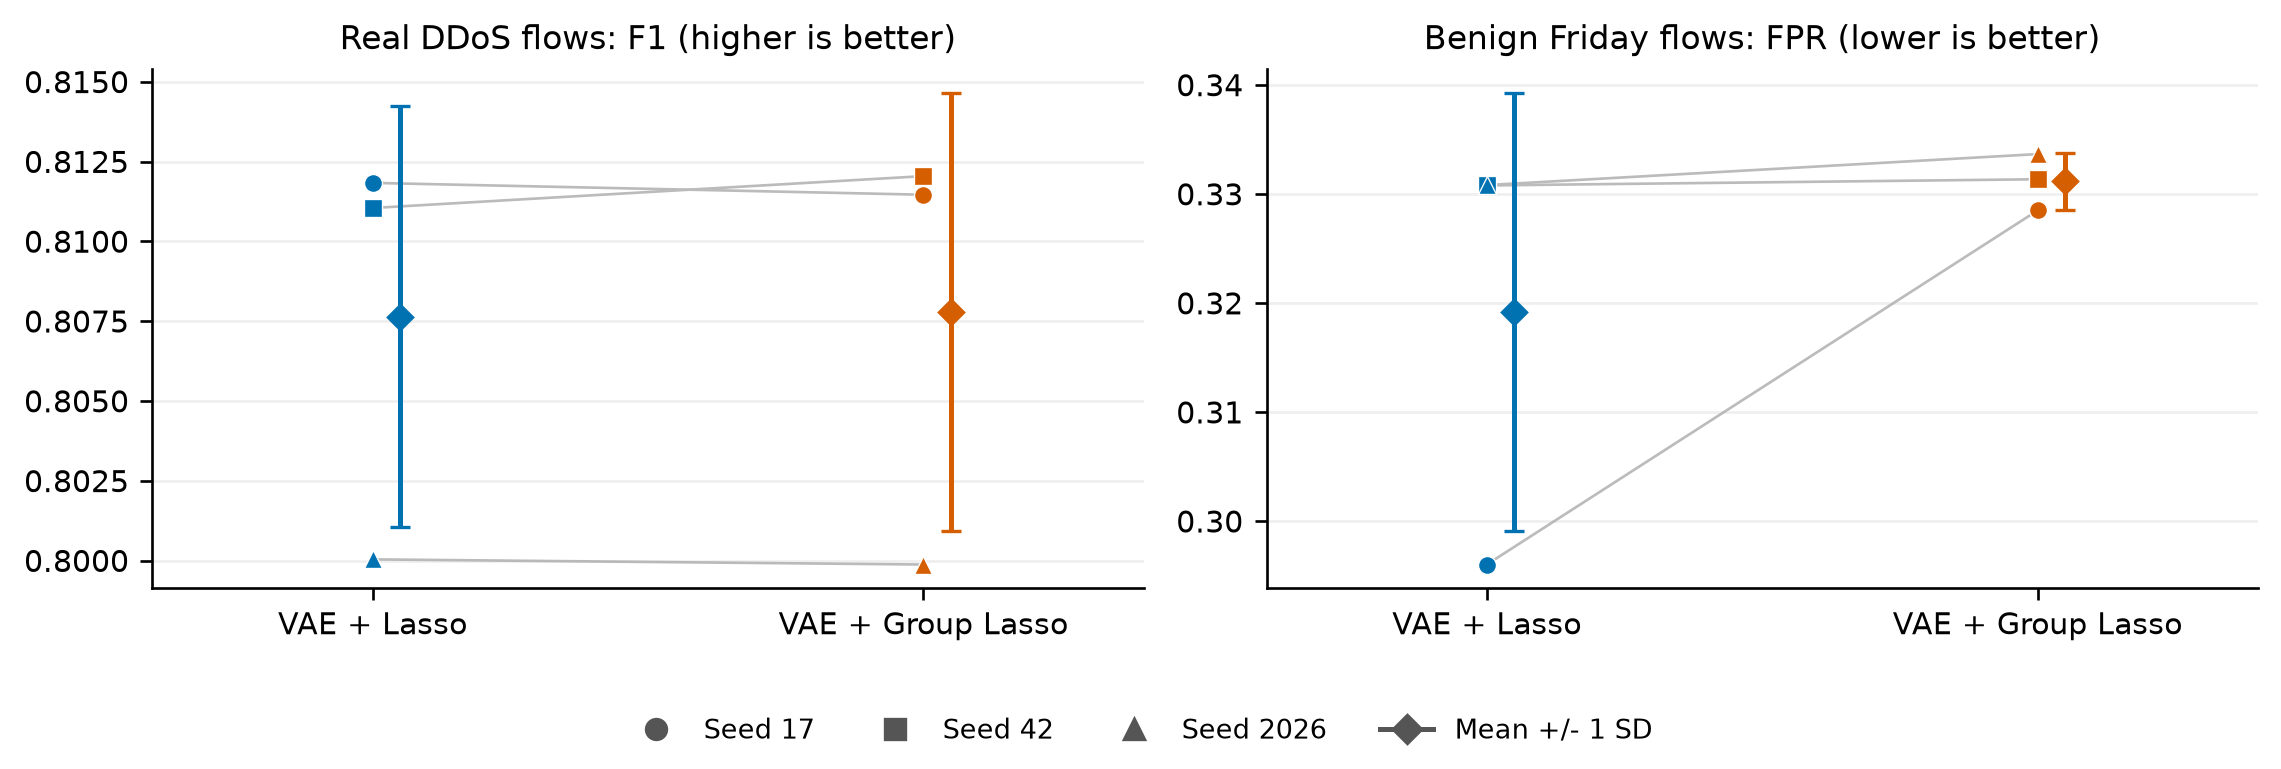
\includegraphics[width=0.98\textwidth]{figures/experiment_03_real_comparison.png}
\caption{Recorded-flow comparison. Circles, squares, and triangles identify
seeds 17, 42, and 2026; diamonds and error bars show the mean and one sample
standard deviation. These are model seeds on one capture, not independent
datasets.}
\label{fig:exp3_real}
\end{figure}

\subsubsection{Routed synthetic traffic: original attacks and matched controls}

We reuse all 15 VAE checkpoints from Experiment 2: three seeds at all five
$\gamma$ values. The topology, nominal signal, noise, and original attack
arrays are unchanged. Groups are the 15 destination nodes, each containing
14 incoming OD flows, defined from topology rather than attack labels.
After normal reconstruction, both decoders receive the identical residual
$r_t=y_t-\hat\ell_t$ and solve
\[
 \min_a\frac12\|r_t-Ra\|_2^2+0.11\mathcal R(a),\qquad
 \mathcal R(a)=\|a\|_1\quad\hbox{or}\quad
 \sum_{g=1}^{15}\sqrt{14}\,\|a_{G_g}\|_2.
\]
The VAE stays frozen; this is a two-stage estimator, not end-to-end training
through a differentiable optimization layer. The fixed penalties and size
weights are specified before evaluation and are not claimed to be optimal.

The third method is the same Algorithm-2 OnlineDA implementation as in
Experiment 2~\cite{Mardani}: rank 5, ridge penalty 0.36, $\ell_1$ penalty
0.11, and forgetting factor 1. It receives the same link observations and $R$,
not VAE residuals. Each test scenario and normal-calibration stream starts from
an independent copy of its normal-trained state. The normal-prefix SVD warm
start remains an explicit adaptation to the paper's random initialization.
OnlineDA adapts causally during testing, whereas the VAE is frozen; this third
comparison is a whole-system benchmark, not an isolated test of the penalty.

Three scenarios distinguish reuse from the new group-structured hypothesis.
\emph{Original independent attacks} are exactly those of Experiment 2.
\emph{Matched dispersed attacks} affect 14 distinct, uniformly sampled flows
at each of 300 randomly selected times. \emph{Destination-grouped attacks}
affect all 14 incoming flows to one randomly selected destination at those
same 300 times. Both matched scenarios use positive unit amplitudes: they
have identical time support, 4,200 attacked cells out of 840,000 (0.5\%), and
OD attack energy. The dispersed control is sampled without replacement at a
fixed count, not by independent Bernoulli draws. Routed link energy can still
differ because paths overlap; it is recorded rather than assumed equal.
New attacks are paired across $\gamma$ within each seed.

Flow and destination-group thresholds use the same 2,000 independent normal
calibration observations as Experiment 2, targeting 1\% FPR separately for
each method and level. Group scores are L2 norms. Zero-score ties make the
achieved calibration FPR conservative, including zero for the grouped decoder
at $\gamma=0$. Average precision (AP) is therefore reported alongside F1.
Compare methods within a scenario: group prevalence differs between scenarios.

\begin{table}[H]
\centering
\caption{Experiment 3: synthetic endpoint means. L denotes VAE+Lasso,
G denotes VAE+Group Lasso, and O denotes OnlineDA. F1 uses normal-calibrated
thresholds.}
\small
\setlength{\tabcolsep}{4pt}
\begin{tabular}{llcccccc}
\toprule
 & & \multicolumn{3}{c}{OD-flow F1} & \multicolumn{3}{c}{OD-flow AP} \\
Scenario & $\gamma$ & L & G & O & L & G & O \\
\midrule
Original independent & 0 & 0.1261 & 0.0335 & 0.5539 & 0.9118 & 0.7905 & 0.9440 \\
Original independent & 1 & 0.1391 & 0.0617 & 0.4163 & 0.8680 & 0.7181 & 0.9295 \\
Matched dispersed & 0 & 0.2160 & 0.1303 & 0.3971 & 0.2545 & 0.3127 & 0.4541 \\
Matched dispersed & 1 & 0.1765 & 0.1280 & 0.2842 & 0.2405 & 0.2839 & 0.4460 \\
Destination grouped & 0 & 0.2956 & 0.1473 & 0.8122 & 0.6652 & 0.9330 & 1.0000 \\
Destination grouped & 1 & 0.2347 & 0.1565 & 0.4949 & 0.4543 & 0.8096 & 0.9998 \\
\bottomrule
\end{tabular}
\label{tab:exp3_synthetic}
\end{table}

\begin{figure}[H]
\centering
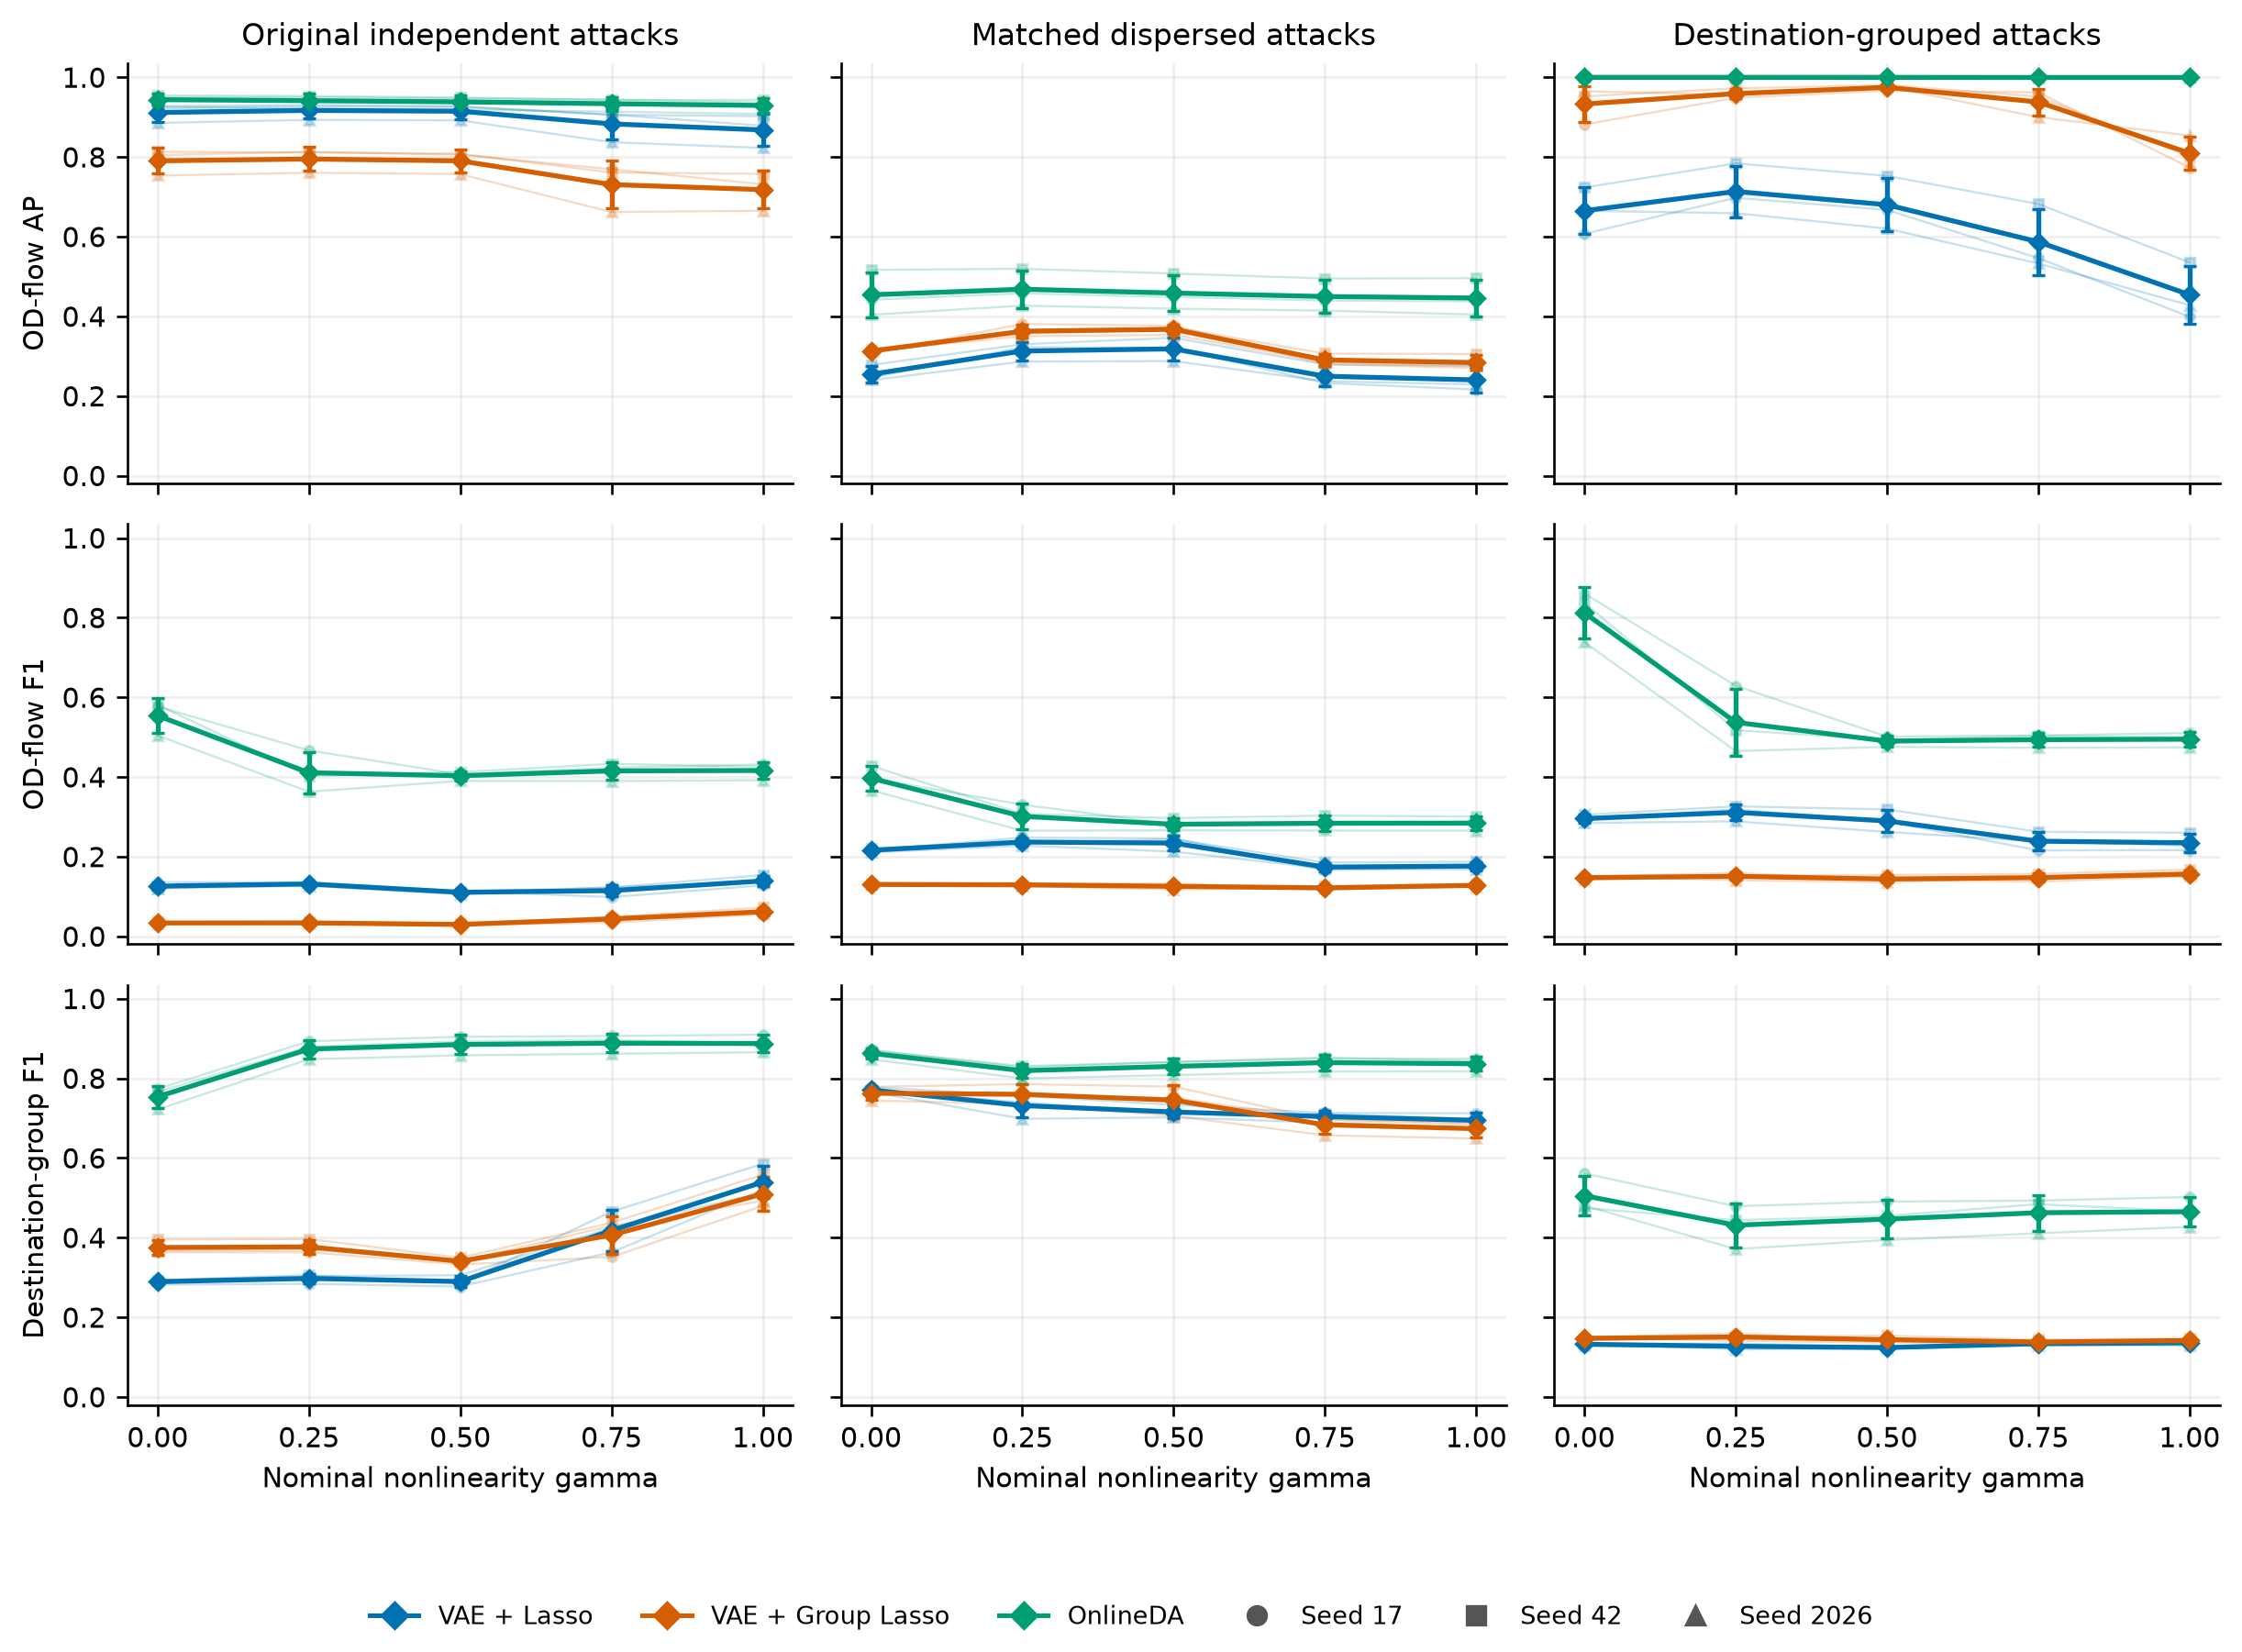
\includegraphics[width=0.98\textwidth]{figures/experiment_03_synthetic_comparison.png}
\caption{VAE+Lasso (blue), VAE+Group Lasso (orange), and OnlineDA (green) at
all five synthetic nonlinearity settings. Rows distinguish flow AP,
flow F1, and destination-group F1; columns distinguish attack structures.
F1 uses normal-calibrated thresholds. Faint seed trajectories use the same
marker identities as Figure~\ref{fig:exp3_real}; diamonds and bars show mean
$\pm$ one sample standard deviation.}
\label{fig:exp3_synthetic}
\end{figure}

On the exact original attacks, Group Lasso has lower flow AP and F1 at every
$\gamma$: grouping is not automatically helpful. On destination-grouped
attacks, however, it improves flow ranking at every $\gamma$. At $\gamma=1$,
AP rises from 0.4543 to 0.8096 and relative OD attack-recovery error falls from
1.1425 to 0.7311. These are genuine ranking and amplitude-recovery gains for
this structured scenario, but they do not translate into higher calibrated
flow F1. The grouped penalty can leave many small nonzero coefficients inside
selected groups, and normal-only thresholds do not necessarily suppress those
false alarms. At the same endpoint, group F1 changes only from 0.1359 to 0.1417.

OnlineDA has higher mean flow F1 and AP than either VAE decoder in all 15
scenario--$\gamma$ settings. On destination-grouped attacks at $\gamma=1$,
its flow F1 is 0.4949, AP is 0.9998, and relative OD recovery error is 0.1894.
Thus the grouped VAE improves on VAE+Lasso in ranking and recovery, but does
not outperform the paper-based online baseline in this experiment.

As a secondary, non-tuned operating point, we also retain the fixed absolute
flow threshold 0.1 already specified in Experiment 2 and the reference protocol.
For destination-grouped attacks at $\gamma=1$, flow F1 is 0.3768 for Lasso and
0.3664 for Group Lasso, versus 0.8268 for OnlineDA. The VAE ranking gain is
not an F1 gain at either reported operating point.

\subsubsection{Numerical verification and scope of the result}

The grouped routing solver uses accelerated proximal gradient with adaptive
restart and an explicit group-KKT residual, not loss stagnation. All 180,000
test and 30,000 distinct normal-calibration subproblems satisfy the normalized
$10^{-5}$ tolerance. Twenty of the 180,000 corresponding test Lasso solves
miss the strict convergence flag, with worst normalized KKT residual
$4.84\times10^{-5}$; these cases remain disclosed in the saved audit.
OnlineDA adds 180,000 test and 30,000 normal-calibration solves; 17 and 8,
respectively, miss the same strict Lasso flag (worst residual below
$4.89\times10^{-5}$). None are dropped. All 15 original test streams and 15
normal-calibration streams reproduce the saved Experiment-2 estimates.
Eighteen unit tests cover block shrinkage, singleton equivalence to Lasso,
a primal-dual gap check, label-independent groups, matched attack budgets,
OnlineDA state restoration, and independent continuous test streams.

Experiment 3 therefore implements an explicit group penalty but finds no
universal improvement: recorded-flow score denoising gives essentially no gain;
routed group structure improves ranking and recovery relative to VAE+Lasso,
but not the tested F1 operating points or the OnlineDA benchmark. Group choice, unequal sizes,
calibration, and the underdetermined routing map remain important limitations.
The real arm uses one laboratory capture, and three seeds do not establish
generalization to independent networks or attacks. Full per-seed results,
sensitivity settings, hashes, and solver diagnostics are retained with the code.

\subsection{Overall Experimental Conclusions}

The three studies separate normal representation, sparse structure, and the
detection operating point. Experiment 1 detects many DDoS flows but suffers
from cross-day false positives. Experiment 2 does not show VAE+Lasso outperforming
the paper's online linear model. Experiment 3 adds a real group penalty: its
benefit relative to VAE+Lasso depends on attack structure and metric, while
OnlineDA remains stronger in synthetic flow F1 and AP. A nonlinear
representation alone does not establish a detection advantage.

The current results support neither universal superiority of VAE+Group Lasso
nor the conclusion that group sparsity is useless. Structured synthetic attacks
show improved ranking and amplitude recovery relative to VAE+Lasso, while thresholded
localization remains weak. A future routing- and mask-conditioned model needs
independent calibration and evaluation on both individual flows and meaningful
groups; group penalties alone do not resolve missing information.

\clearpage
% We now use the 'alpha' style for formal, letter-based citations (e.g., [BDE09])
\bibliographystyle{alpha}
\bibliography{references}

\end{document}
